\documentclass[output=paper]{langsci/langscibook}
\ChapterDOI{10.5281/zenodo.4545029}
%\documentclass[output=paper,colorlinks,citecolor=brown]{langscibook}


\title[Multi-modal estimation of cognitive load in post-editing of MT]
      {Multi-modal estimation of cognitive load in post-editing of machine translation}

\author{Nico Herbig\affiliation{German Research Center for Artificial Intelligence (DFKI); Saarland University; Saarland Informatics Campus} and Santanu Pal\affiliation{German Research Center for Artificial Intelligence (DFKI); Saarland University; Saarland Informatics Campus} and Antonio Krüger\affiliation{German Research Center for Artificial Intelligence (DFKI); Saarland University; Saarland Informatics Campus} and Josef van Genabith\affiliation{German Research Center for Artificial Intelligence (DFKI); Saarland University; Saarland Informatics Campus}}


\abstract{In this paper, we analyze a wide range of physiological, behavioral, performance, and subjective measures to estimate cognitive load (CL) during post-editing (PE) of machine translated (MT) text. To the best of our knowledge, the analyzed feature set comprises the most diverse set of features from a variety of modalities that has been investigated in the translation domain to date.
Our focus lies on predicting the subjectively reported perceived CL based on the other measures,
%in order to quantify the extent of demands placed on the mental resources available during PE. This
which could for example be used to better capture the usefulness of MT proposals for PE, including the mental effort required, or to develop cognition-aware translation environments that support human translators according to their current level of CL.
Based on the data gathered from 10 professional translators, we show that feature sets from all different modalities outperform our baseline measures in terms of predicting the subjectively perceived level of CL, and that especially eye-, heart-, or skin-based features yield good results in a simple ``top-down'' regression analysis using feature selection. When passing the participant and segment to the regression models, other modalities like keyboard, text, body posture, or time, also perform well.
An additional correlation analysis provides insights into redundancies among the features which may be used to further improve the currently achieved best regression score of 0.7 mean squared error (MSE) on a 9-point scale.}
% An investigation of correlations between the best performing features, including features previously unexplored in PE, shows which feature sets capture similar or distinct underlying concepts. Furthermore, the correlation analysis shows promising insights that may be used for creating predictive models which potentially even further improve the currently achieved best regression score of 0.7 mean squared error (MSE) on a 9-point scale.}

\begin{document}
\renewcommand{\lsChapterFooterSize}{\footnotesize}
\maketitle

\section{Introduction}
Even though machine translation (MT) systems are improving rapidly, the resulting translations currently still require manual post-editing (PE) to capture and correct errors and make the target texts conform to their intended objective. PE has the potential of inducing high cognitive load (CL) on the translator: it involves continuous scanning of texts, including source, the incrementally evolving final translation output and possible error-prone MT output for mistakes, \mbox{(sub-)strings} that can be reused, text that has already been translated, text that still needs to be translated, etc. When PE is required, we should therefore optimize for a low perceived CL during PE, and not only focus on MT quality in terms of automatic measures or time to post-edit. Here, we see CL as ``a variable that attempts to quantify the extent of demands placed by a task on the mental resources we have at our disposal'' \citep{chen2016robust}.

While CL and MT quality are interrelated, they cannot be considered equal: for example, repeated mistakes that have been corrected by the translator again and again in the past may impact perceived CL, while the MT quality remains the same. Therefore, it has been argued that CL is a more decisive indicator of the overall effort expended by post-editors  \citep{vieira2016measures}.

To investigate how computer-aided translation (CAT) tools could adapt when high cognitive loads are detected, \citet{herbig2019chi} interviewed professional translators. The most proposed and most liked idea was to provide alternative translations from MT, translation memories (TM), or a corpus; however, other adaptations like automatic proposals to encourage the translator to take a break, reordering segments to switch between highly and less demanding segments, user interface adaptations, or payment based on induced CL were also discussed.

Apart from these CAT adaptations based on CL, the automatic capture of CL without interfering in the PE process would further enable the creation of large datasets of CL scores for (source, MT, PE) tuples that could be used to optimize MT systems to produce output inducing lower CL on the post-editors.

% Contributions
To provide some first steps towards these goals, we are concerned with the question of how to actually estimate CL during PE. For this,
(1) we present an approach based on a wide range of physiological, behavioral, performance, and subjective measures, yielding the so far most diverse set of features from a variety of modalities that has been investigated in the translation domain.
(2) We analyze how well predictive models based on feature combinations from these modalities can predict perceived CL, as measured by subjective ratings on a well established CL scale from psychology \citep{paas1994instructional}. The different modalities and their combinations are then compared in terms of regression performance.
(3) Similar to \citet{vieira2016measures}, we investigate pairwise correlations between different interesting indicators of CL and also subjectively assessed CL and run a principal component analysis (PCA) to figure out which features capture similar or distinct underlying concepts. This step aims to help us understand the relation between the different CL estimators.

% Summary of findings
The results of our analyses indicate that heart, eye and skin, as well as combined measures perform very well on their own, while text, keyboard, body posture, or time features only perform well when considering the individual participant and segment they are editing. Overall, the best predictive model achieved a regression score of 0.7 mean squared error (MSE) on a 9-point scale. However, the correlation analysis shows that our ``top-down'' approach to regression analysis, which uses a simple feature selection algorithm, sometimes chooses redundant features, suggesting that it might be possible to improve results by analyzing the features in more depth and combining them in a more sophisticated way.

\section{Related work}
This section discusses related studies by first giving an overview of CL measures and then presenting studies on %the causes of CL and the
measuring CL during translation.

\subsection{Overview of cognitive load measures}
Cognitive load theory \citep{paas1994instructional, sweller1998cognitive} has been developed in psychology and is concerned with an efficient use of people's limited cognitive resources to apply acquired knowledge and skills to new situations \citep{paas2003cognitive}. Approaches to detect CL can be roughly divided into four categories: subjective measures, performance measures, behavioral measures, and physiological measures.

% Subjective measures
\textsc{subjective measures} are based on the assumption that subjects can self-as\-sess and report their cognitive processes after performing a task \citep{paas1994instructional}. Several scales exist, and introspection is often used as a ground truth to evaluate how well CL can be assessed by other means, such as physiological measurements.

%Performance measures
\textsc{performance measures} such as the time required or the text quality achieved assume that when working memory capacity is overloaded, a performance drop occurs due to the increase in overall CL \citep{chen2016robust}. However, by increasing their efforts, humans can compensate for the overload and maintain their performance over a period of time, although this can lead to additional strain and fatigue \citep{hockey1997compensatory}.

% Behavioral measures
\textsc{behavioral measures} can be extracted from user activity while performing a task. Especially interesting in the context of PE are mouse and keyboard input-based features, which were shown to correlate to CL \citep{arshad2013analysing}.

% Physiological measures
Last, a lot of research has been done on \textsc{physiological measurements}, which assume that human cognitive processes can be observed in the human physiology \citep{kramer1991physiological}.
% Eyes
Eye-tracking is frequently used for physiological CL measurements: the pupil diameter increases with higher CL \citep{iqbal2004task,obrien_eye-tracking_2006}, the frequency of rapid dilations changes \citep{demberg2016frequency}, and the blink behavior adapts \citep{van2001eye}. Furthermore, \citet{chen2013automatic} as well as \citet{stuyven2000effect} showed that fixations and saccades can also be used for CL predictions.
% Skin
Apart from the eyes, the skin also provides information about the user's cognitive state: galvanic skin response (GSR) can be used to determine whether a user feels stressed \citep{villarejo2012stress} and provides information about the CL \citep{shi2007galvanic}. Remote measurements of the skin temperature have also been effective \citep{yamakoshi2008feasibility}.
% Heart
Further commonly used indicators rely on the cardiovascular system: blood pressure \citep{yamakoshi2008feasibility}, heart rate \citep{mulder1992measurement}, and especially heart rate variability (HRV; \citealp{rowe1998heart}) have been shown to correlate with CL.
% Others
%Other physiological measures include respiration \citep{chanel2008boredom} and brain activity \citep{hosseini2010emotional,solovey2012brainput}.
%Combinations of such brain activity measures, eye based measures, and subjective measures have also been explored in the context of subtitle processing in movies \citep{kruger2016measuring,kruger2018multimodal}.
%Furthermore, the recent improvements in computer vision using deep learning allow automatic extraction of emotions from videos \citep{kahou2016emonets}.
In addition, simple features such as the head pose also correlate to CL when learning \citep{asteriadis2009estimation}.

%\subsection{What Leads to Cognitive Effort During Translation?}
% What leads to effort?
%The question of which sentence features affect PE effort has been researched as well.

%\cite{tatsumi2009correlation} analyzed the relation between automatic evaluation scores and PE speed and found that especially the source sentence length and structure yield to longer PE times.
%\cite{temnikova2010cognitive} extended an existing MT error classification by ranking the error types in terms of cognitive effort based on a cognitive model of reading, working memory theory, and written error detection studies.
%However, an analysis of which CL these errors actually induce on editors was not performed.
%\cite{koponen2012comparing} compared edit distances to human judgments specifying the amount of PE effort that would be necessary to achieve a useful translation. Similar scales were also proposed by \cite{specia2010machine} and \cite{callison2010findings}, measuring quality/expected percentage that needs editing and implicitly assuming this to be equal to CL.
%\cite{koponen2012post} ``suggest post-editing time as a way to assess some of the cognitive effort involved in post-editing''.
%\cite{lacruz2014chapter} correlate different error types, classified into mechanical and transfer errors, to a typing behavior metric ($\mathrm{PWR}$, see below), $\mathrm{HTER}$ \citep{TER:2006,TERp:2009}, and user ratings of MT quality. Similarly, the work of \cite{popovic2014relations} shows that ``lexical and word order edit operations require most cognitive effort, lexical errors require most time, while removing additions has low impact on both quality and on time''; however, they simply considered human quality level scores indicative of cognitive effort.

%To summarize, these works provide insight into which features of a MT output lead to longer PE times or worse subjective quality ratings; however, a direct link to CL in the psychological sense was not shown, but only assumed to exist.

\subsection{Cognitive load estimation in the translation domain}
Due to the parallel activation of two languages, reading for translation imposes more demand on the working memory than reading within a single language \citep{macizo2006reading}, thus, making CL estimation particularly interesting in the translation domain. Therefore, a few, albeit seminal, publications relevant to the cognitive dimension of modeling PE have been presented:

% Think aloud protocols
\citet{krings2001repairing} utilized think-aloud protocols to capture cognitive effort; however, as pointed out by \citet{o2005methodologies}, post-editors constantly reporting what they are doing (a) slows down the process and (b) changes the process itself.

% Pauses / Typing
\citet{o2005methodologies} explored correlating pauses in typing behavior to potentially difficult source text features. In a follow-up analysis \citep{o2006pauses}, she concluded that ``while pauses provide some indication of cognitive processing, supplementary methods are required''. % to give a fuller picture''.
\citet{lacruz2012average} and \citet{lacruz2014chapter} built upon this work, but instead of examining long pauses, they analyzed clusters of shorter pauses. Their metrics called average pause ratio (\apr{}) and pause to word ratio (\pwr{}) could be correlated to technical effort (the required mouse and keyboard actions), arguing that ``it is likely that in many situations technical effort and cognitive effort will be related''. Pause ratios were also shown to be more sensitive to grammatical, word order, or structure errors.
For TMs, \citet{mellinger2014computer} was able to correlate keystroke logs and pause metrics to translation quality ratings.
Last, when post-editing, the total pause duration was found to be smaller than during manual translation of metaphors  \citep{koglin2015empirical}; however, this could be explained by the large time savings achieved through PE.

While pauses relate to these MT quality measures and technical effort, which are most likely related to perceived CL, they cannot be considered equal: consider very bad MT proposals that are still very easy to PE due to the simplicity of the segments or the contrary situation, a very high MT quality where spotting the error can remain difficult and induce a high CL. We will nevertheless integrate pause measures, as they are very easily applicable in TPR studies, but compare them to physiological and subjective measures of CL.


% Eye-tracking
Among the physiological measures, eye-tracking has frequently been used as a means to capture CL during PE:
\citet{obrien_eye-tracking_2006} proposed pupil dilation as a measure of CL and focused on correlations with different match types retrieved from a TM.
\citet{doherty2010eye} also explored eye-tracking by measuring different features while reading MT output. They found that gaze time and fixation count correlate with MT quality; however, fixation duration and pupil dilation were less reliable.
\citet{carl2011process} found more fixations and longer gaze times on the target text when comparing PE to manual translation. Therefore, the authors argue that there is more effort in correcting MT outputs, whereas manual translation requires more effort for reading and understanding the source. This finding was also replicated by \citet{koglin2015empirical}.
\citet{moorkens_correlations_2015} correlated ratings of expected PE effort with temporal, technical and cognitive effort, in terms of time, translation error rate ($\mathrm{TER}$; \citealp{TER:2006,TERp:2009}), and fixation counts and durations, respectively. Interestingly, the correlations between eye-tracking data and predicted effort were either very weak or weak, suggesting that human predictions of PE effort cannot be considered completely reliable.
Furthermore, \citet{daems2016translation} found that fixations are mostly impacted by coherence and other meaning shifts.
In contrast to these quality-, time-, and expectation-based measures, \citet{vieira2014indices} uses a psychology-motivated definition of CL. He linked average fixation duration, fixation counts, and a self-report scale measuring CL, which is frequently used in psychology \citep{paas1994instructional} to segments expected to pose different levels of translation difficulty and their corresponding Meteor \citep{Lavie:2007} ratings.

As can be seen, a variety of approaches already exists linking different eye features to effort metrics, ranging from simply counting fixations on the source and target to pupil diameter measures. However, the focus was again mostly on a link to translation quality, sentence features, or expected effort, with only one consideration of CL in the psychological sense. Furthermore, the works only investigated eye tracking, without considering other physiological or behavioral measures.

% Most relevant works
In contrast, the follow-up work by \citet{vieira2016measures} analyzes how all of the above measures, as well as pause metrics and editing time, relate to each other in a multivariate analysis. He found correlations between all measures; however, a PCA showed that they cluster in different ways.
The work most related to this study is our previous study -- \cite{herbig2019mt} -- with translation master's students, where we explored a vast variety of CL measures, including eye, skin, heart, and typing features that were previously unexplored in the translation domain, analyzed correlations, and investigated how well these can be used to predict the subjective CL ratings.

In this work, we built upon our previous findings (1) by conducting a similar study with professional translators instead of translation master's students, (2) by incorporating even more sensors and features in the system, and (3) by not only analyzing predictive models of subjective CL or correlations to this subjective measure, but further by performing the multivariate analysis of \citet{vieira2016measures} to understand how the different measures relate to each other and how the features cluster together.


\section{Method}
As stated earlier, we believe that the CL perceived by translators during PE should be considered more closely, since MT output often requires PE, and considering only the number of changes needed may not provide an accurate measure of the effort involved \citep{koponen2016machine}. %By focusing on the CL during PE, we aim for improved motivation to work and avoidance of boredom, exhaustion and stress.
Adding this CL-based perspective on PE of MT to the commonly used but oversimplifying BLEU  \citep{BLEU:2002} perspective on MT quality should lead to a better approximation of actual PE cost.
%
%Thus, we need a method to robustly measure CL in PE. As we have seen in the related works section, plenty of approaches to estimate CL have been proposed in a variety of domains and some factors have even been tested in translation studies. %However, the question remains which of the related approaches are applicable for detecting CL when PE of MT, since several metrics have not been evaluated at all for PE or were only linked to MT quality.

To test which measuring approaches can actually reflect different levels of CL in PE, we perform a user study\footnote{The study was approved by the university's ethical review board% and the data protection officer
.} to gather data from a variety of sensors, which can be combined in a multi-modal fashion.
For the analysis, we conduct a hybrid of the approaches by \citet{herbig2019mt} and \citet{vieira2016measures}. That is, we aim to predict subjectively assessed CL based on the captured multi-modal sensor data by training regression models and we further perform a multivariate analysis and a PCA to find pairwise correlations and clusters of different features.
The goal of the regression analysis is to be able to automatically infer the CL from the raw sensor data, ideally using as few and as commonly used sensors as possible%, to avoid interruptions by asking for these ratings
. The multivariate analysis should then provide more detailed insights into why some measuring approaches perform well while others contribute little.

\subsection{Analyzed measures of cognitive load}
\label{sec:CLmeasures}
Compared to \citet{vieira2016measures}, \citet{herbig2019mt} already increased the amount of analyzed features significantly by adding heart-, skin-, and camera-based features. In this work, we add even more and higher quality sensors and add further high-level features.

% Subjective
\subsubsection{Subjective measures}
Subjective measures are based on the assumption that subjects can self-assess and report their cognitive processes after performing a task. For this, we adapted a CAT tool to ask for a subjective CL rating (\subjCL{}) using the scale proposed by \citet{paas1994instructional} after every single segment. This scale was chosen because it focuses on CL and not on quality, %has been widely used and verified in many application areas,
and further since it was used in the two most related studies by \citet{vieira2016measures} and \citet{herbig2019mt}. %, can be answered quickly as it contains only a single question (in contrast to NASA-TLX \citep{hart1988development}), and allows ratings on a 9-point scale, thereby offering a sufficiently wide range to select from.
The single 9-point question is ``In solving or studying the preceding problem I invested'' with a choice of answers ranging from ``very, very low mental effort'' to ``very, very high mental effort''.

% Performance/ Text/Time
\subsubsection{Performance measures: Text and time}
The usual performance measures based on the required time or achieved quality are not as easily accessible in PE as in other cognitive tasks, since it is possible to trade of quality for time and because translation quality is a partly subjective measure.  Nevertheless, we integrate the following simple time and text measures:

For the \herbigemph{{time features}} we integrate PE time (\petime{}) and length-normalized PE time which also considers the segment length (\lnpetime{}).

The \herbigemph{{text features}} consist of smoothed \bleu{}, \hbleu{} \citep{Lin:2004:AEM:1218955.1219032}, \ter{}, \hter{} \citep{TERp:2009}, and sentence length (\sentencelength{}).
Note that the difference between the non-H- and H-based measures lies in the choice of the reference translation and hypothesis: \bleu{} and \ter{} take the MT output as hypothesis and the independently provided human translation as reference and calculate $n$-gram overlap (BLEU) or the amount of necessary edits (TER) to transform the hypothesis into the reference, while \hbleu{} and \hter{} perform the same calculations, but this time between the MT output and the post-edited translation.

% Behavioral
\subsubsection{Behavioral measures: Keyboard typing and body posture}
Behavioral measures can be extracted from user activity while performing a task. Especially interesting in the context of PE, where the translator does not move a lot, is focused on the screen, does not speak, etc., are \herbigemph{{mouse and keyboard input-based features}}. Therefore, our most basic sensor is a key logger storing all keyboard and mouse input during PE. The higher-level pause features \apr{} and \pwr{} by \citet{lacruz2012average}, which were shown to correlate with PE effort, are automatically calculated from the keyboard events.

% Emotions
% We further add a webcam to record images at a fixed interval which we use to estimate basic emotions based on a trained neural network available through a Microsoft API.

% Body Posture
Furthermore, the \herbigemph{{body posture}} is captured by a Microsoft Kinect v2. We hypothesize that post-editors come closer to the screen for hard-to-edit translations, so we calculate the distance to the head and normalize it per participant (\headdist{}).


% Physiological
\subsubsection{Physiological measures: Eyes, heart, and skin}
As physiological measurements, we integrate eye-, heart-, and skin-based measures in our experiment.


% Eyes
For \herbigemph{{eye-based features}}, we use a web-cam and an eye tracker. The web-cam, which is naturally not as precise as the eye tracker but easily accessible on most modern devices, is used to calculate the eye aspect ratio (\ear{}), which indicates the openness of the lids \citep{soukupova2016real}.
The remote Tobii eye tracker 4C with the Pro SDK records the raw gaze data. Based on this raw data, we calculate the amount of blinking (of less than 2\,s length; \blinkamount{}) and also normalize this by the PE time (\normblinkamount{})  \citep{van2001eye}. Similarly, we calculate the number of fixations (\fixamount{}) and normalize it by PE time (\normfixamount{}).
We further compute the fixation durations (\fixdur{}) and saccade durations (\saccdur{})  \citep{doherty2010eye,moorkens_correlations_2015}, all of which have been shown to be indicators of CL.
Furthermore, we reimplemented the work by \citet{goldberg1999computer} to calculate the probability of visual search based on the eye movements (\searchprob{}), which was proposed to determine whether a user is searching within a user interface and could therefore also be an indication of a user feeling ``lost'' while PE.
Last, and as the main distinction from \citet{herbig2019mt}, we also capture the pupil diameter (\rawpupil{}, \citealt{obrien_eye-tracking_2006}). For calculating higher-level features on the sensor output, we first replace blinks from the signal by linear interpolation. Then, the index of cognitive activity (\ica{}{}), which is the frequency of small rapid dilations of the pupil \citep{demberg2016frequency} that was shown to be more robust to changes in illumination, is calculated based on this signal. Two approaches are implemented: one uses a wavelet transformation to calculate the number of rapid dilations (\ica{wave}{}), while the other simply counts how often a sample deviates by more than 5 times the rolling standard deviation from the rolling mean of the signal (\ica{count}{}).
Last, we also implemented the work of \citet{hossain2014understanding}, which checks for sharp changes and continuations of the ramp in the Hilbert unwrapped phase of the pupil diameter signal (\hilbert{}).


% Heart
For \herbigemph{{heart measures}}, we integrate three devices: a Polar H7 heart belt, a Garmin Forerunner 935 sports watch, and the Empatica E4 wristband. That way, we have two sports devices (Polar and Garmin) and one CE certified medical device (type 2a) offering an early glimpse of the data quality achieved by future consumer devices. %Furthermore, we can compare the two wrist-worn devices (Empatica and Garmin) to the chest-worn measurements by the Polar belt.
From both the Polar belt and the Garmin watch, we capture the heart rate (\hr{}{}).

The Polar belt, as well as the Empatica wristband, further capture the RR interval (\rr{}{}), which is the length between two successive Rs (basically the peaks) in the ECG signal.
Based on this, we calculate the often-used CL measures of heart rate variability (HRV, \citealt{rowe1998heart}), in particular the root mean square of successive RR interval differences (\rmssd{}{}) and the standard deviation of NN intervals (\sdnn{}{}). Here, the \sdnn{}{} uses NN intervals, which normalize across the RR intervals and thereby smooth abnormal values.
Furthermore, we add the HRV features \nn{}{} and \pnn{}{}, which are the number and percentage of successive NN intervals that differ by more than 50\,ms \citep{shaffer2017overview}, for both the Empatica and the Polar to the analysis.

Furthermore, the Empatica measures the blood volume pulse (\bvpempatica{}), which is the change in volume of blood measured over time. Based on it, we calculate the BVP amplitude (\bvpamplitudeempatica{}, \citealt{iani2004effects}), which contains the amplitude between the lowest (diastolic point) and highest (systolic point) peak in a one second interval. Last, we also calculate the median absolute deviation (BVPMed\-AbsDev) and the mean absolute difference (\bvpmeanadempatica{}) among the BVP values \citep{haapalainen2010psycho}. Here, \bvpmedadempatica{} is the median of the absolute differences between individual measurements and the median of all measurements. \bvpmeanadempatica{} is simply the mean of absolute differences of each pair of measurements. Both these features are calculated per interval of 125\,ms.

The main difference compared to \citet{herbig2019mt} regarding heart features is that we additionally included the Garmin and Empatica devices, which allowed us to also integrate BVP-related measures. Furthermore, we extended the set of considered HRV measures to also include \nn{}{} and \pnn{}{}.


% Skin
% Empatica in microsiemens
% MSBand in Kilo Ohm
For \herbigemph{{skin-based features}}, we integrate the Microsoft Band v2 and again use the Empatica and the Garmin devices.
The MSBand and Empatica both measure the commonly used galvanic skin response (\gsr{}{}) which is an indicator of CL. We also transform this signal to the frequency domain (\freqgsr{}{}) as described in \cite{chen2016robust}. In accord with their work, we also calculate data frames of length 16, 32, and 64 samples, which are similarly transformed to the frequency domain and normalized by the participant average (\freqframegsr{}{}).

Furthermore, we use the Ledalab software\footnote{\url{http://www.ledalab.de/}} to calculate higher level skin conductance features on the Empatica raw data. It provides us with ``global'' features, namely the mean value (\ledalabGlMean{}) and the maximum positive deflection (\ledalabGlMaxDefl{}), and ``through-to-peak (TTP)/min-max'' analysis, namely the number of significant (i.e.\ above-threshold) skin conductance responses (SCRs)\linebreak (\ledalabttpnscr{}), the sum of SCR amplitudes (\ledalabttpampsum{}) of significant SCRs, and the response latency (\ledalabttplatency{}) of the first significant SCR. Furthermore, and most interestingly, we use Ledalab to perform a continuous decomposition analysis (CDA, \citealt{benedek2010ledalabCDA}), which separates skin conductance data into continuous signals of tonic (background) and phasic (rapid) activity.
%This method extracts the phasic (driver) information underlying EDA, and aims at retrieving the signal characteristics of the underlying sudomotor nerve activity (SNA). SC data is deconvolved by the general response shape which results in a large increase of temporal precision. Then data is decomposed into continuous phasic and tonic components (Benedek & Kaernbach, 2010b). It features the computation of several standard measures of phasic EDA. Moreover, straightforward measures such as the average (or integrated) phasic driver activity are provided.
The features based on this CDA analysis again include the number of significant SCRs, the SCR amplitudes of significant SCRs, and the latency of the first SCR (\ledalabcdanscr{}, \ledalabcdaampsum{}, \ledalabcdalatency{}). Furthermore, the average phasic driver (\ledalabcdascr{}), the area of phasic driver (\ledalabcdaiscr{}), as well as the maximum value of phasic activity (\ledalabcdaPhasicMax{}) and the mean tonic activity (\ledalabcdaTonic{}) features are created by the Ledalab software.

% Skin temperature
The Empatica and Garmin devices also measure the skin temperature, which we use as a feature (\skintemp{}{}). %Furthermore, the Garmin Forerunner 935 also has a built-in temperature sensor which we use (\skintemp{Garmin}{}).

The differences from \citet{herbig2019mt} for the skin features are as follows: we further use the skin resistance data delivered by the Empatica E4 wristband, on which we calculate the same features as in their work, but additionally add the Ledalab features. Furthermore, we integrate the skin temperature features.


% Why no EEG, two-finger GSR, wearable eye trackers etc.
%One should note that all sensors included in our analysis do not significantly hinder the translation process or feel uncomfortable. This is also the reason why we did not include two-finger GSR sensors, head-mounted eye trackers, or EEG sensors.

% Normalization and transform from signal to indiv. feature
\subsubsection{Data normalization and segment-wise feature calculation}
\label{sec:datanorm}
The features described above can be categorized into two classes: \textit{global features} and \textit{continuous features}.

By \textsc{global features} we mean features that yield only one value per segment: this class comprises subjective measures (\subjCL{}), time measures (\petime{}, \lnpetime{}), text measures (\bleu{}, \hbleu{}, \ter{}, \hter{}, \sentencelength{}), keyboard measures (\apr{}, \pwr{}), the amount-based eye features (\blinkamount{}, \fixamount{}, Norm\-Blink\-Amount, \normfixamount{}), and all Ledalab skin features. However, one should note that the time and text features here really only can be calculated on the whole segment, while the amount-based eye features or the skin-based Ledalab features could also be calculated over shorter periods of time.

Apart from these global features, all other features are basically just a \textsc{continuous signal} (of different sampling rates) that we still need to transform to a directly usable set of values per segment.
Each signal is first normalized as described in \cite{chen2016robust} by dividing it by the participant's mean value. Then 6 very simple features are calculated from this normalized signal: the accumulated, average, standard deviation, minimum, maximum, and range ($\max - \min$). As an example, this means that \gsr{}{}, actually consists of the 6 features \gsr{}{acc}, \gsr{}{avg}, \gsr{}{std}, \gsr{}{min}, \gsr{}{max}, and \gsr{}{range}.

% Data filtering
We manually inspected the data distribution per segment and participant for outliers and overall data quality. First of all, the Empatica E4 sensor, which claims clinical quality observations, indeed shows the fewest outliers and nicely bell shaped data distributions. In contrast, the Polar H7 sports sensor and the Microsoft Band v2 showed much more noisy data. Therefore, we filtered values according to visual inspection and related literature: data above 100,000\,kΩ for the raw MSBand GSR was removed. Furthermore, Polar \rmssd{}{} and \sdnn{}{} values above 1000 \citep{van2018normal} as well as \hr{Polar}{} and \rr{Polar}{} samples which fall outside the acceptable 50--120 beats per minute or 500--1200\,ms ranges were ignored \citep{shaffer2017overview}.

\subsection{Text and apparatus used for the experiment}
% Which text
Apart from the sensors, we need to generate translations for our experiments that contain realistic error types. For this, we use the same 30 sentences as \citet{herbig2019mt}, which are chosen as follows: % and also randomize the sentence order to avoid ordering effects.
a neural MT system \citep{Gehring:2017:fair} was trained on the English-German parallel data from the WMT 2017 news translation task and provided translation candidates on the respective test data set. % where it achieved a test score of 29.5 in \bleu{} and 60.1 in \ter{}.
Then 30 sentences were chosen from this test set by (a) using sentences of different \ter{} intervals, (b) reducing the possible candidates based on manual error analysis, and (c) further shrinking the set based on subjective CL ratings from two translation master's students in a pre-study. For details regarding the selection of sentences please refer to \cite{herbig2019mt}.
All participants used these same 30 segments; however, the order is randomized to avoid ordering effects. %While using WMT data, which consists of independent segments instead of complete texts, prevents us from analyzing the effects of textual (i.e.\ cross-sentential) coherence and cohesion on CL, it allows us to perform this randomization of segment order which would not make sense with a complete text. Since each participant receives the same segments in a different order, potential effects such as feeling tired towards the end of the experiment do not always affect the same segments, and therefore balance out.

% More text pieces in case we want to extend
% (a)
%After using our NMT system, we extracted 300 sentences and their translations, 100 each within different $\mathrm{TER}$ score intervals\footnote{As $\mathrm{TER}$ intervals we used [35-50], [60-70], and [80-95].}. All segments had a length of $\leq 35$ words.
% (b)
%Out of these 300 sentences, we extracted 60 segments based on error rules to ensure different difficulties are represented in this set. For this, we categorized the errors contained as being either errors of lexical choice, containing mistranslated words or errors in fluency, or errors in word order. By selecting sentences containing these error types and combinations thereof, we hoped to induce different levels of CL on the participants.
% (c)
% To further reduce the amount of segments and to ensure that these actually can cause different levels of CL on the participants, we performed a pre-study (with counterbalanced segment order). Two German natives with a similar English skill level, as both are in the same translation science master's program, participated and translated the 60 segments. As described above, a pop-up appeared after each segment asking for a subjective CL rating. We used the resulting 2 times 60 segment ratings to pick 30 for the final study. For this selection, we filtered out segments with disagreement \textgreater 3 on the 9-point Likert scale, meaning that they had at least a similar judgment. To pick 30  sentences, the remaining sentences were ordered by average rating, and we removed multiple segments with equal average ratings to achieve an equal rating spread. The hope was that this well-distributed set of CL perceptions among the participants of this pre-study leads to transferable ratings in the final study. Note however, that we did not use the pre-study ratings as the CL labels for the following actual study, but only to perform this pre-selection of segments. In the main study we again ask the participants for CL ratings, and use their individual ratings for the analysis to capture inter-participant differences.


%\subsection{Apparatus}
For the study, the post-editor is equipped with a Microsoft Band v2 on her right wrist, the Garmin Forerunner 935 and Empatica E4 on the left wrist (the Garmin is further up), the heart belt on her chest, and an eye tracker, as well a web-cam and a Microsoft Kinect v2 camera facing her. As input possibilities, a standard keyboard and mouse are attached, and a 24-inch monitor displays the SDL Trados Studio 2017 translation environment. We chose Trados for this study as it is by far the most used CAT tool in professional applications.

\subsection{Data analysis approach}
% Intro: multi step etc
%We analyze the gathered data in a multi-step approach:
First, we analyze the subjective ratings provided by our participants% and how we filtered the raw sensor data (see Section~\ref{sec:SubRate})
.
Then, similar to \citet{herbig2019mt}, we estimate the subjective ratings of perceived CL %(cf.\ Section~\ref{sec:method-regression})
based on a combination of different features.
Last, we use the approach by \citet{vieira2016measures} and investigate correlations between our measures %eye, pause, and time features
to understand how they relate to each other% and how they cluster together. One should note here that we analyze many more features than \cite{vieira2016measures}, so we aim to both reproduce and extend his findings (see Section~\ref{sec:corr:PCA})
.

For all analyses, we discuss the features in terms of the feature sets described in Section~\ref{sec:CLmeasures}: \textit{subjective}, \textit{time}, \textit{text}, \textit{keyboard}, \textit{body posture}, \textit{heart}, \textit{eye}, and \textit{skin} features. Finally, we also investigate \textit{combinations} of these sets.

% Subjective Ratings, Do sensors actually measure the same thing when they say so?
\subsubsection{Subjective ratings}
\label{sec:SubRate}
We start by reporting and analyzing the subjective ratings provided by our participants. As this is our target measure, it is important to understand the distribution of our dataset as well as inter-rater differences.
%As a small and initial side investigation, we report correlations between measures produced by different sensors, e.g. how similar is data captured by an actual heart belt compared to wrist-based heart measurements, that would be easily applicable in practice?
% We further describe how outliers were removed from our dataset. While this does not directly relate to estimating CL when PE, it might help researchers and practitioners decide which sensors to use and which filters to apply.

% Regression: all features, each category, different target features, which models used, etc. 10 by 1 and 5 by 2 fold CV
\subsubsection{Multi-modal CL regression analysis}
\label{sec:method-regression}
The goal of this stage is to investigate the feasibility of automatically gathering CL values for segments through different sensors. For this, we learn a function that fits our features to the subjective CL as reported by each participant on the rating scale after each segment; thus, the output space is 1 to 9. We consider each segment of each participant an individual sample with the corresponding subjective rating as a label. Please note that neither a manual annotation of the segments nor an average CL rating across participants is used here.

% Why subjective as baseline
The reason why we focus on subjectively assessed CL is that it is good at capturing inter-translator differences% in contrast to any general measure of quality
. This is important because the task difficulty by itself is of a subjective nature, as it depends on the translator's experience with similar texts, vocabulary, etc. %; hence, the translations are not objectively hard or easy.
% Ordinal output vs continuous output
%Please note that the rating scale used \citep{paas1994instructional} is ordinal; however, the outputs of our regressors are continuous. The reason is that we explicitly decided to use the scale as it was designed and verified without any alterations, but did not see value in forcing the models to output ordinals because their target value, CL, spans a continuous space.
Thus, we also do not normalize our target variable, because the lowest rating assigned by one participant is not necessarily comparable to the lowest rating assigned by another participant due to prior experience, which in turn could also result in different physiological responses.
Thus, instead of potentially biasing our data by transforming the target variable, we keep it as is and perform a comparison between models with a random effect for participant and those without such knowledge, as described in further detail below.
Apart from subjectively assessed CL we could also have chosen quality or time measures as the target, however, as discussed above, quality and CL cannot be considered equal, and time could be traded off for quality, thereby limiting findings based solely on these measures.

% Baselines
We compare the different regression models based on different feature sets against each other, but also compare each model to a very simple baseline: always predicting the mean subjective rating (\baselineCLmean{}).

% Regression models
Overall, we compare two approaches for training regression models.

The first approach uses only the above measures to predict \subjCL{}, and has no knowledge about which participant the data comes from or which segment was post-edited while recording the data. Thus, it is a very generic approach that learns one set of parameters across all participants, thereby exploring the feasibility of applying CL adaptations during PE in practice, e.g.\ for automatically providing alternative proposals when loaded.
Since different features and their combinations require different types of functions to best approximate them locally% (e.g.\ not all of them show linear relations)
, we train not only one, but several regression algorithms making different assumptions about the underlying function space:
linear models with different regularizers, namely a stochastic gradient descent regressor (SGD), a lasso model (Lasso), an elastic net (ENet), and a ridge regressor (Ridge), as well as a non-linear random forest regressor (RF), all provided in the \texttt{scikit-learn} library using the default parameters and feature normalization. This analysis is very similar to \citet{herbig2019mt}, except that our previous analysis additionally used a support vector regression (SVR) model.\footnote{Since SVR does not support our selected feature selection approach, and since it never performed best in tests without feature selection, we decided to not use it for this experiment.}

As a second approach, which is an extension to the first approach, we further integrate linear mixed-effect models (LMEMs) using R (version 3.6.0, \texttt{lme4} package version 1.1-21), as these can effectively capture inter-participant as well as segment-dependent differences by adding a random effect for subject and  a random effect for item.\footnote{Since the R package used for LMEMs does not support our feature selection approach either, we decided to instead perform feature selection with a normal linear regression model with L2 regularization.} To make the comparison between LMEMs and the other models fair, we also provide the \texttt{scikit} models with the participant and segment ID; thus, all models can learn to act differently depending on this information. While the normalization of the signal discussed above already normalizes the data such that each participant's average heart rate is at value 1, some participants might still react more strongly to CL, e.g.\ one participant might increase his heart rate by 10\%, while another's might increase by 20\%. By incorporating the participant and segment as a feature into the models, we ensure that they can learn such individual difference. This is also a major distinction from \citet{herbig2019mt}, who did not incorporate these measures. However, this approach of training the models is only relevant for strictly controlled experiments, because in practice no two translators will PE the same segment.

By training multiple regression models, we obtain locally optimal results before comparing them and drawing conclusions on the usefulness of the features involved. That way, our results are not biased or distorted by the use and limitations of a single classifier (and with it the class of functions that can be learned). While we do not fine-tune hyper-parameters of the models and might therefore miss some ideal hyper-parameter combination, our approach offers a reasonably wide range of function spaces to choose from.

% Implementation Details
To avoid over-fitting, all regression functions use regularization or averaging, and we perform cross-validation (CV).
% Missing data values for features are replaced by the mean of the feature values across all participants and segments\todo{how often did this happen?}. --> Not at all, just had the code there from a pre-study
Before passing a feature to a regression model, we apply a z-transformation to achieve 0 mean and unit variance.
For combining individual features within a modality or across modalities, we then use simple vector concatenation.
As a feature selection approach we use recursive feature elimination with CV (\texttt{RFECV} in \texttt{scikit-learn}) to decide on the amount of features to select.

% Cross validation
For all of these feature combinations, we train each of the above regressors using a 10-fold stratified CV, which is better suited for an imbalanced distribution of the target variable (that we happen to have, see Section~\ref{sec:subjRatings}).
We further perform a 5 by 2-fold stratified CV which we use to statistically compare the different models. This method has been suggested by \citet{dietterich1998approximate} as it ensures that each sample only occurs in the train or test dataset for each estimation of model skill, thereby reducing inter-dependencies. Naturally, every regression model is trained on the same folds, to make results comparable.
For each regressor, the average test MSE is computed across the 10 folds and is then compared across regressors as it is a good measure for our actual goal: predicting the subjective CL as well as possible. We choose the MSE as the main metric, since the error squaring strongly penalizes large errors, which are particularly undesirable for our goal.

% Pairwise correlation + PCA of interesting feature sets
\subsubsection{Pairwise correlations and PCA}
\label{sec:corr:PCA}
\citet{vieira2016measures} argues that ``using a large number of different measures in the hope that together they will provide a more accurate parameter might be an inefficient appraoch'', especially when the measures are correlated. Our above approach uses a well established feature selection mechanism to select a good feature subset and thereby automatically reduces redundancies and removes inconclusive features. However, this ``top-down'' experimental approach still does not provide any insight into how all the different features correlate and which features reflect the same underlying construct. %Furthermore, the above regression naturally is only interested in correlations to subjective CL, which we selected as our target variable, and is not concerned with correlations between different features themselves.

To target these shortcomings, \citet{vieira2016measures} inspects a correlation matrix visualizing pairwise feature correlations. To further investigate why some measures seem to be more related to each other than others, suggesting that there is also a great degree of redundancy involved, he then used a PCA. As \citet{vieira2016measures} nicely puts it, ``informally, PCA transforms a group of variables into a group of orthogonal principal components (PC) containing linear combinations of the original variables''. Usually a small number of PCs is enough to explain most of the original data, which is especially important for our data consisting of a huge amount of features.

To keep the reporting concise, we only report PCs that together explain 95\% of the variance%, i.e.\ components capturing less then 5\% variance are not plotted
.
Since we have many more features than \citet{vieira2016measures}, a plot including all features would become very messy and unreadable. Therefore, we create a separate plot per modality to investigate within-modality correlations and further report an across-modality plot. For modalities with more than 5 features, we reduce this set based on the MSE a regressor that was trained solely on each single feature would achieve in a 5 by 2-fold CV. While this does not give us a full picture, it remains interpretable and provides interesting insights.

\subsection{Participants and user evaluation procedure}
The experiment participants were 10 professional translators (8 female), aged 28--62 ($\text{mean}=40.4, \SD=9.7$). Half of them were freelance translators, while the other half worked for a translation company. All of them were native Germans and had studied translation from English. Their professional experience ranged from 3 to 30 years ($\text{mean}=12.1, \SD=3$). All of them have worked with Trados SDL Studio, which is the CAT tool we also used for our experiment. However, on average they have used 4.4 distinct CAT tools ($\SD=2.1, \min=1, \max=9$). On a 5-point scale ranging from very bad to very good, they judged their knowledge of CAT tools as good ($\text{mean}=4.2, \SD=0.9$), their experience with Trados as good ($\text{mean}=4.4, \SD=0.7$), their general knowledge of translation as very good ($\text{mean}=4.8, \SD=0.4$), and their PE knowledge as good ($\text{mean}=3.8, \SD=1.0$).

%Apart from filling out a basic questionnaire gathering the above demographics and signing a data protection form prior to the experiment,
After signing a data protection form and filling out the above demographics questionnaire, they were given written instructions explaining that they should (1) post-edit the proposed translations and not translate from scratch, and (2) focus on grammatical and semantic correctness while avoiding stylistic changes. Concrete time limits were not stated. The reason for clear instructions was to ensure a similar PE process across participants; other specifications would also have been valid for such an experiment.
We further allowed but did not require participants to look up terms in a corpus or dictionary online. Before starting the actual PE process, they were given time to familiarize themselves with the environment, e.g.\ to adjust the chair and adapt the Trados view settings.
They then each post-edited the 30 text segments described above in random order while wearing all the sensors.
For one participant the USB hub we used broke after post-editing 9 segments, thereby reducing the gathered amount of data for this participant.

\section{Results and discussion}\largerpage
In this section, we present and discuss the results of each individual step of our data analysis.

\subsection{Subjective ratings}\label{sec:subjRatings}

% rating distribution
All 9 CL ratings were used during the experiment; however, 90.3\% of the ratings were within the range 3 to 7 (inclusive) while the extreme cases were only rarely chosen (see Figure~\ref{fig:segments_by_rating}).
% inter-rater differences
We also observe rating differences between post-editors, with an average standard deviation across segments of 1.2 %(minimum 0.8, maximum 1.8)
on our 9-point scale. %When asked after the experiment how demanding it was overall, i.e.\ a retrospective overall judgement, the scores are very much in line with the ratings given immediately after each segment, with a mean of 5.4 and a standard deviation of 0.8.
% comparison to journal
In general, the rating distribution and the inter-rater differences are strongly comparable to the results of \citet{herbig2019mt}.
As argued in this work, a reason for the non-uniform, rather normal rating distribution could be the strong wording of the used rating scale \citep{paas1994instructional}: ``very, very high/low mental effort'' is something that we believe users simply do not identify themselves with often.
%Even though we invested work in finding segments that we expected to induce very, very low or high mental effort through the pre-study, the inter-personal differences seem to simply be too high to ensure this.
%These inter-personal rating differences also show why CL and the BLEU perspective of MT quality cannot be considered equal, since the latter is an objective measure, while perceived CL is an inherently subjective variable and depends on how individuals cope with variation in the demands of a task \citep{vieira2016measures}.

\begin{figure}
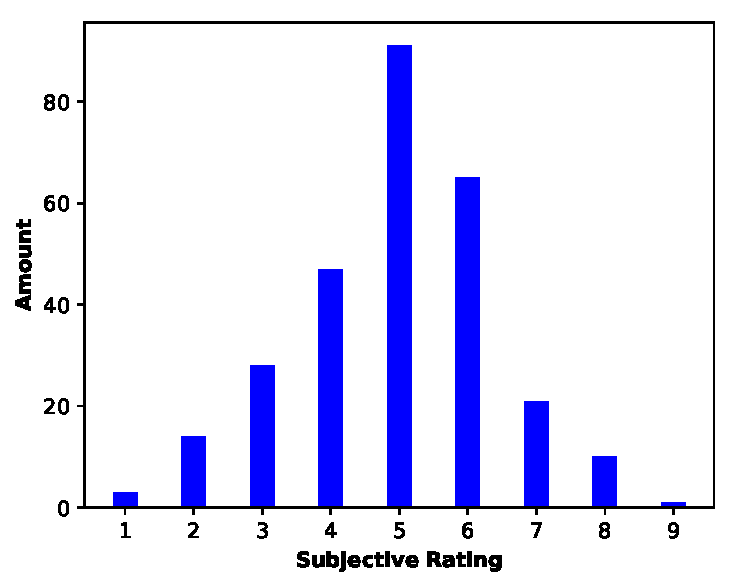
\includegraphics[scale=0.5]{figures/rating_dist.pdf}
\caption{Rating distribution across subjective CL scale.\label{fig:segments_by_rating}}
\end{figure}

Note that we use these individual CL ratings (without any aggregation on segment level) for the remaining analyses to also capture inter-participant differences.
Inspecting the data in further detail, we find %34 out of 197 cases where multiple participants rated the same segment as equally tough while having an editing difference of more than 30 \hbleu{}. Analogously,
80 out of 151 cases where multiple participants rated the same segment as equally tough while having an editing difference of more than 20 \hter{}. This supports our above argument that strong differences in editing behavior do not necessarily impact the CL.

%\subsubsection{Sensor Correlations}
%We further investigated correlations between measures produced by different sensors. The results can be seen in Table~\ref{tab:sensor-correlations}. While the heart rate and temperature measures indeed correlate strongly, they still do not match exactly. We expected this, since measuring at different positions and using different sensors will never give exactly the same results. What we did not expect however, is that the RR intervals by the Empatica and Polar belt are only correlated to a medium extend. We do assume the Empatica data to be of high quality as achieved several regulatory compliances and was designed as a research device instead of for mere sports purposes. However, since the Polar device is worn at the chest, we had expected it to produce rather accurate measures as well even though it is only a sports device.


%\begin{table}[h]
%
%\begin{tabular}{llll}
%\midrule
%\textbf{Feature}      & \textbf{Spearm.'s $\rho$, p} & \textbf{Pearson's $\rho$, p} & \textbf{Interpret.}  \\
%\midrule
%\midrule
%\rr{Empatica}{} vs.\ \rr{Polar}{}     & $0.38$, $<0.01$                          & $0.32$, $<0.01$ & Medium \\
%\hr{Garmin}{} vs.\ \hr{Polar}{}     & $0.81$, $<0.01$                          & $0.71$, $<0.01$ & Strong \\
%\skintemp{Garmin}{} vs.\ \skintemp{Empatica}{}     & $0.83$, $<0.01$                          & $0.74$, $<0.01$ & Strong \\
%\midrule
%\end{tabular}
%\caption{Spearman's correlation results between different features and subjective CL ratings.}
%\label{tab:sensor-correlations}
%\end{table}

\subsection{Multi-modal CL regression analysis}\largerpage
The results of the first regression analysis approach, that is \textit{without passing the participant and segment} alongside the features to the model, are reported in Table~\ref{tab:resultsnopartid}.
It shows the MSE achieved in 1 by 10- and 5 by 2-fold CV, once for the baseline, and further for each category of features described above. For each feature category, we report the results achieved by a model trained on all features (ALL) of that category, and the results achieved by a model trained using feature selection (FS). The features are ordered by their regression performance (MSE) when training a model solely on this single feature. %, as this is one (among many) measures of what this feature contributes.
Next to each MSE score, we report the type of model (e.g.\ Ridge). Last, we also report the standard deviation of the 10 runs within 5 by 2-fold CV.

The first thing one should note when looking at Table~\ref{tab:resultsnopartid} is that only ridge and random forest models were chosen, and that the results for 1 by 10-fold and 5 by 2-fold CVs are rather similar. %, although the latter is often slightly worse.
We compare each 5 by 2-fold MSE score using a univariate ANOVA with all models as conditions and calculate the contrasts to the mean baseline as references. The ANOVAs violated the sphericity assumption but still showed strong significance ($p<0.01$) after Greenhouse-Geisser correction of the degrees of freedom. Table~\ref{tab:resultsnopartid} shows that all models are significantly better than the mean baseline (after Bonferroni correction).

When looking at the individual results in Table~\ref{tab:resultsnopartid}, one can see that already this baseline is actually quite good, with a MSE of 2.045 on a 9-point scale, which comes from the rather normally distributed ratings. Among our considered categories, text is the worst, followed by keyboard, body posture, and time, which show similar results. Much better and more interesting results are obtained in the three categories skin, eye, and heart measures, which again show similar results. When combining multiple modalities, the results improve a bit further.


\begin{table}
\footnotesize
	\begin{tabularx}{\textwidth}{l@{~~}Q@{}r@{~~}r}
		\lsptoprule
		&&  \multicolumn{2}{c}{{MSE}} \\\cmidrule{3-4}
&{Features} & {1x10-CV}$\downarrow${(Reg.)}  & {5x2-CV}$\downarrow$ {(SD)}\\
\midrule

{Baseline}
& \baselineCLmean{} & 2.045 (-) & 2.045 (0.04) \\
\midrule

{Time Features}
&ALL: \petime{}, \lnpetime{}	& 1.457 (Ridge) & 1.487 (Ridge) (0.11)*\\
&FS: \petime{} & 1.453 (Ridge) & 1.490 (Ridge) (0.11)*\\
\midrule

{Text Features}
&ALL: \ter{}, \hter{}, \hbleu{}, \bleu{}, \sentencelength{} & 1.756 (Ridge) & 1.764 (Ridge) (0.07)*\\
&FS: \ter{}, \hter{}, \sentencelength{} & 1.736 (Ridge) & 1.747 (Ridge) (0.07)*\\
\midrule

{Keyboard}
&ALL: \pwr{}, \apr{} & 1.551 (Ridge) & 1.577 (Ridge) (0.08)*\\
&FS: \pwr{} & 1.554 (Ridge) & 1.568 (Ridge) (0.07)*\\
\midrule

{Body Posture}
&ALL: \headdist{} & 1.471 (Ridge) & 1.487 (RF) (0.11)*\\
&FS: \headdist{} & 1.456 (Ridge) & 1.474 (RF) (0.12)*\\
\midrule

{Eyes}
&ALL: \searchprob{}, \fixamount{}, \ica{}{}, \fixdur{}, \saccdur{}, \hilbert{}, \ear{}, \blinkamount{}, \rawpupil{}, \normfixamount{}, \normblinkamount{} & 0.965 (RF) & 1.086 (RF) (0.08)*\\
&FS: \fixamount{}, \ica{}{}, \fixdur{}, \saccdur{}, \searchprob{}, \hilbert{}, \ear{}, \rawpupil{} & 0.918 (RF) & 1.029 (RF) (0.09)*\\
\midrule


{Heart}
&ALL: \nn{}{}, \pnn{}{}, \bvpmedadempatica{}, \hr{}{}, \sdnn{}{}, \rmssd{}{}, \rr{}{}, \bvpmeanadempatica{}, \bvpamplitudeempatica{}, \bvpempatica{} & 1.073 (RF) & 1.130 (RF) (0.13)*\\
&FS: \bvpmedadempatica{}, \nn{}{}, \sdnn{}{}, \rmssd{}{}, \hr{}{}, \rr{}{}, \bvpamplitudeempatica{}, \bvpempatica{} & 1.004 (RF) & 1.117 (RF) (0.11)*\\
\midrule
{Skin}
&ALL: \skintemp{}, \ledalab{}, \freqframegsr{}{}, \gsr{}{}, \freqgsr{}{} & 0.942 (RF) & 1.148 (RF) (0.17)*\\
&FS: \skintemp{}{}, \freqframegsr{}{}, \ledalab{}, \gsr{}{}& 0.858 (RF) & 1.033 (RF) (0.14)*\\
\midrule

{Combined Features}
&ALL & 0.857 (RF) & 0.984 (RF) (0.15)*\\
&FS: \fixamount{}, \ica{}{}, \saccdur{}, \nn{}{}, \sdnn{}{}, \fixdur{}, \rmssd{}{}, \freqframegsr{}{}, \hr{}{}, \headdist{}, \ledalab{}, \searchprob{}, \hilbert{}, \skintemp{}{}, \ear{}, \gsr{}{}, \rawpupil{} & 0.718 (RF) & 0.886 (RF) (0.12)*\\
\lspbottomrule
\end{tabularx}
\caption{Feature evaluation results \textit{without considering LMEMs/without adding participant and segment}. For 10-fold and 5 by 2-fold CV with standard deviation (SD). Asterisk (*) in the right column indicates a significant difference ($p<0.01$) from \baselineCLmean{} after Bonferroni correction.\label{tab:resultsnopartid}}
\end{table}


Table~\ref{tab:resultspartid} shows how the results change when including LMEMs %to the list of potential regressors,
and \textit{adding the participant and segment} as additional features to the other regression models. %This allows the trained models to react differently to different participants and segments, thereby losing generality but allowing better model fits.
%
This time only LMEMs and random forest models were chosen, and again the 1 by 10-fold and 5 by 2-fold scores are roughly comparable. %, with the 5x2 scores being slightly worse.
We again use a univariate ANOVA (including Greenhouse-Geisser correction) % due to a violation of sphericity)
and find that all models are significantly better than the baseline (after Bonferroni correction).

When comparing the results of Table~\ref{tab:resultspartid} to Table~\ref{tab:resultsnopartid}, we see that the results with participant and segment improved substantially for the time, text, keyboard, and body posture categories. For the other modalities -- eyes, heart, skin, as well as combinations -- the results are roughly comparable. Even though the performance improved, the text features remain the worst category, followed by the keyboard features. All other modalities now show similar results.

\begin{table}
\footnotesize
	\begin{tabularx}{\textwidth}{l@{~~}Q@{}rr}
		\lsptoprule
		&& \multicolumn{2}{c}{{MSE (L: LMEM, R: RF)}} \\
\cmidrule{3-4}

&{{Features}} & {1x10-CV}$\downarrow${(Reg.)}  & {5x2-CV}$\downarrow$ {(SD)}\\
\midrule
{Baseline}
& \baselineCLmean{} & 2.045 (-) & 2.045 (0.04) \\
\midrule
{Time Features}
&ALL: \petime{}, \lnpetime{}	& 0.856 (L) & 0.886 (L) (0.04)*\\
&FS: \petime{} & 0.868 (L) & 0.891 (L) (0.05)*\\
\midrule
{Text Features}
&ALL: \ter{}, \hter{}, \hbleu{}, \bleu{}, \sentencelength{} & 1.126 (L) & 1.219 (L) (0.07)*\\
&FS: \ter{}, \hter{}, \sentencelength{} & 1.121 (L) & 1.193 (L) (0.04)*\\
\midrule
{Keyboard}
&ALL: \pwr{}, \apr{} & 1.075 (L) & 1.158 (L) (0.06)*\\
&FS: \pwr{} & 1.055 (L) & 1.136 (L) (0.06)*\\
\midrule
{Body Posture}
&ALL: \headdist{} & 0.890 (L) & 0.963 (L) (0.06)*\\
&FS: \headdist{} & 0.872 (L) & 0.896 (L) (0.05)*\\
\midrule
{Eyes}
&ALL:\searchprob{}, \fixamount{}, \ica{}{}, \fixdur{}, \saccdur{}, \hilbert{}, \ear{}, \blinkamount{}, \rawpupil{}, \normfixamount{}, \normblinkamount{} & 0.924 (R) & 0.968 (R) (0.07)*\\
&FS: \fixdur{}, \searchprob{} & 0.882 (R) & 0.938 (L) (0.09)*\\
\midrule
{Heart}
& ALL: \nn{}{}, \pnn{}{}, \bvpmedadempatica{}, \hr{}{}, \sdnn{}{}, \rmssd{}{}, \rr{}{}, \bvpmeanadempatica{}, \bvpamplitudeempatica{}, \bvpempatica{} & 0.921 (R) & 1.057 (R) (0.11)*\\
& FS: \hr{}{} & 0.820 (L) & 0.859 (L) (0.06)*\\
\midrule
{Skin}
& ALL: \skintemp{}, \ledalab{}, \freqframegsr{}{}, \gsr{}{}, \freqgsr{}{} & 0.860 (R) & 1.018 (R) (0.16)*\\
& FS: \skintemp{}{}, \gsr{}{} & 0.816 (L) & 0.919 (L) (0.16)*\\
\midrule
{Combined Features}
&ALL & 0.801 (R) & 0.962 (R) (0.12)*\\
& \fixamount{}, \ica{}{}, \saccdur{}, \nn{}{}, \sdnn{}{}, \fixdur{}, \rmssd{}{}, \freqframegsr{}{}, \hr{}{}, \headdist{}, \ledalab{}, \searchprob{}, \hilbert{}, \skintemp{}{}, \ear{}, \gsr{}{}, \rawpupil{} & 0.703 (R) & 0.867 (R) (0.13)*\\
\lspbottomrule
\end{tabularx}
\caption{Feature evaluation results when \textit{considering LMEMs/adding participant and segment}. For 10-fold and 5 by 2-fold CV with standard deviation (SD). Asterisk (*) in the right column indicates a significant difference ($p<0.01$) from \baselineCLmean{} after Bonferroni correction.\label{tab:resultspartid}}
\end{table}


%Apart from comparing the models against the baselines, w
We also perform pairwise comparisons between the feature selection models of each individual category against the feature selected version of \textit{combinations}, which we report in Table~\ref{tab:pairwise}. Note that these results are using the models without incorporating participant and segment (Table~\ref{tab:resultsnopartid}), as we found these results more interesting. For the pairwise comparisons we use the 5 by 2-fold CV results in combination with a modified $t$-test \citep{dietterich1998approximate} followed by Bonferroni-Holm corrections.

As expected, the \textit{combined} model is indeed significantly better than \textit{time}, \textit{text}, \textit{keyboard}, and \textit{body posture}; however, it is not significantly better compared to \textit{eyes}, \textit{heart}, and \textit{skin}, which are already very good by themselves.

\begin{table}
\begin{tabular}{lr@{ }c}
\lsptoprule
Features & \multicolumn{1}{c}{$\tilde{t}$} & \\
\midrule
Time vs.\ combined & $-4.06$ & *\\
Text vs.\ combined & $-6.03$ & *\\
Keyboard vs.\ combined & $-5.35$ & *\\
Body posture vs.\ combined & $-6.32$ & *\\
\midrule
Eyes vs.\ combined & $-0.98$& \\
Heart vs.\ combined & $-1.42$& \\
Skin vs.\ combined & $-1.34$& \\
\lspbottomrule
\end{tabular}
\caption{Pairwise comparisons between the feature selected models without LMEM\slash without participant and segment (Table~\ref{tab:resultsnopartid}). * shows significance with $p<0.05$ after Bonferroni-Holm correction. $\tilde{t}$ is the test statistics for the modified paired $t$-test \citep{dietterich1998approximate}.\label{tab:pairwise}}
\end{table}

Summarizing, Tables~\ref{tab:resultsnopartid} and \ref{tab:pairwise} suggest that CL measurement without special adaptations per participant and segment work best when combining multiple modalities; however, using skin, eye, or heart measures also works similarly well. The often used keyboard features based on typing pauses, as well as time and body posture measures perform worse. The text metrics, which include common quality measures, are the worst among our explored predictors of subjective CL.

When the models can adapt to participant and segment (Table~\ref{tab:resultspartid}), the often used text and keyboard features remain the worst; however, all other categories (time, body posture, eyes, heart, skin, as well as combinations) now perform similarly well.

\subsection{Pairwise correlations and PCA}
Similar to \citet{vieira2016measures}, we analyze pairwise correlations between our measures of CL. For each modality, we report a maximum of 5 best features, which we compare to each other and to the subjective rating.

\begin{figure}
    \begin{subfigure}[b]{0.5\textwidth}\centering
        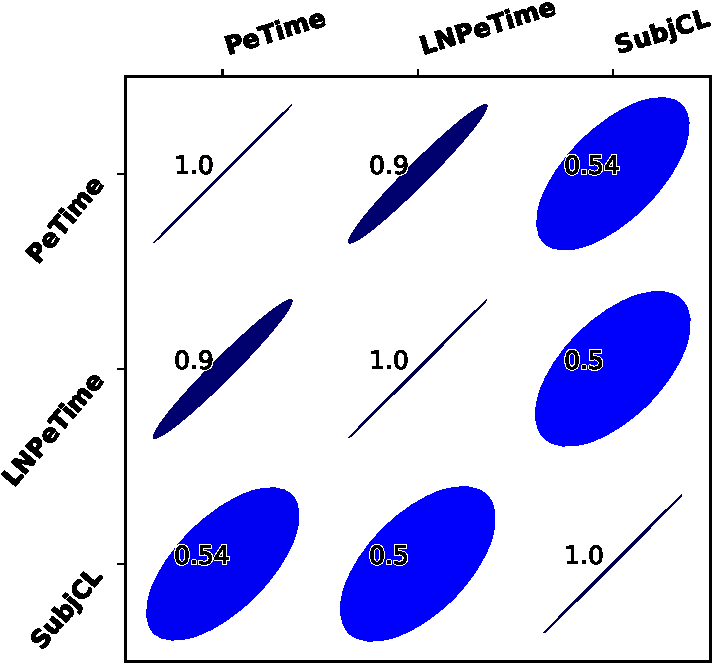
\includegraphics[height=4.5cm]{figures/time-pearson-cropped.pdf}
        \caption{Time -- Pearson}
    \end{subfigure}%
    \begin{subfigure}[b]{0.5\textwidth}\centering
        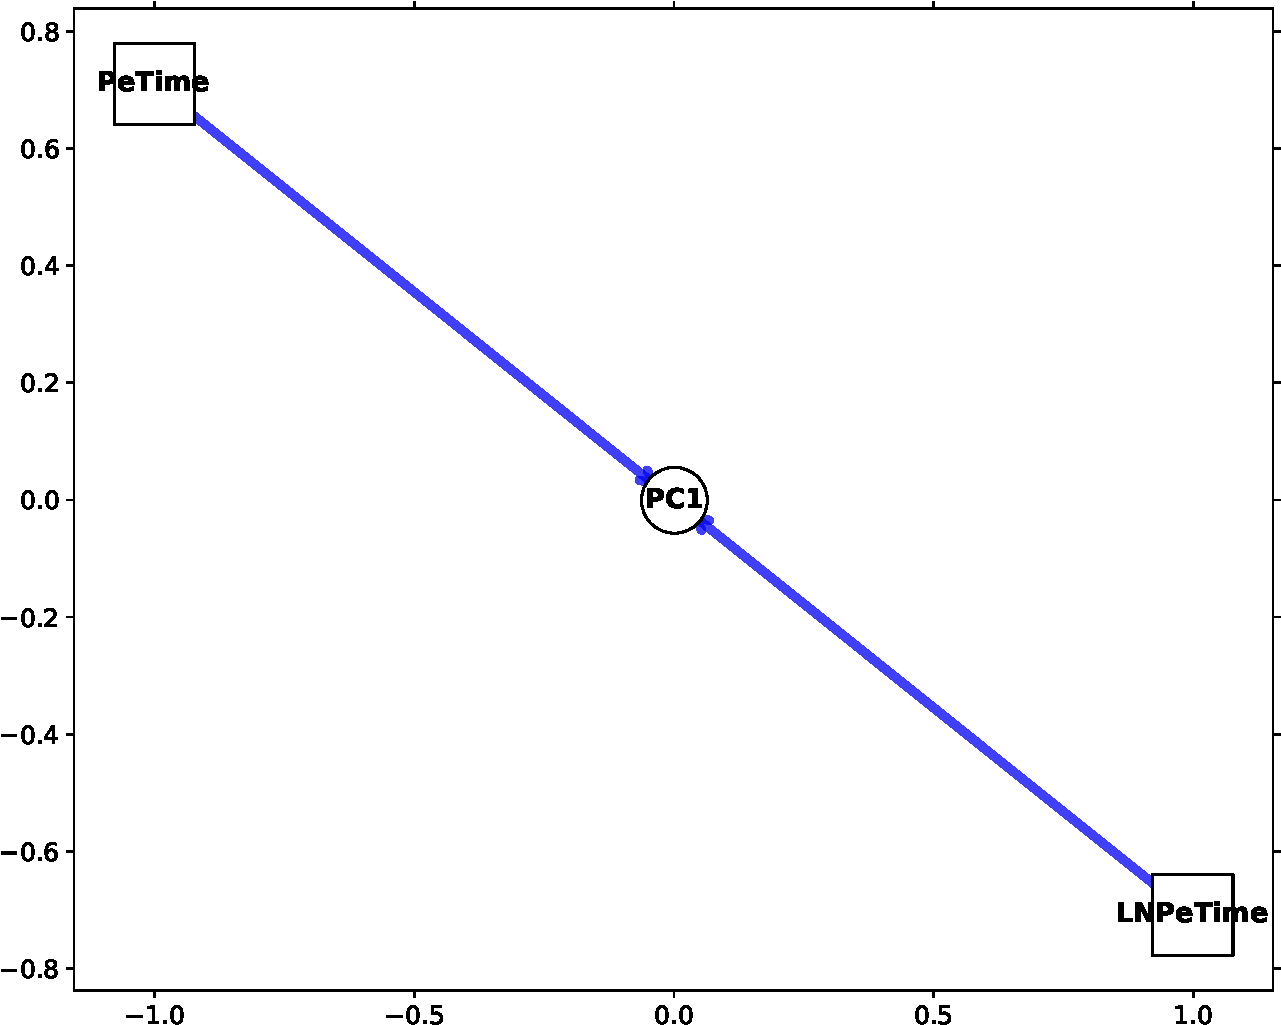
\includegraphics[height=4.5cm]{figures/time-PCA-cropped.pdf}
        \caption{Time -- PCA}
    \end{subfigure}\bigskip\\
    \begin{subfigure}[b]{0.5\textwidth}\centering
        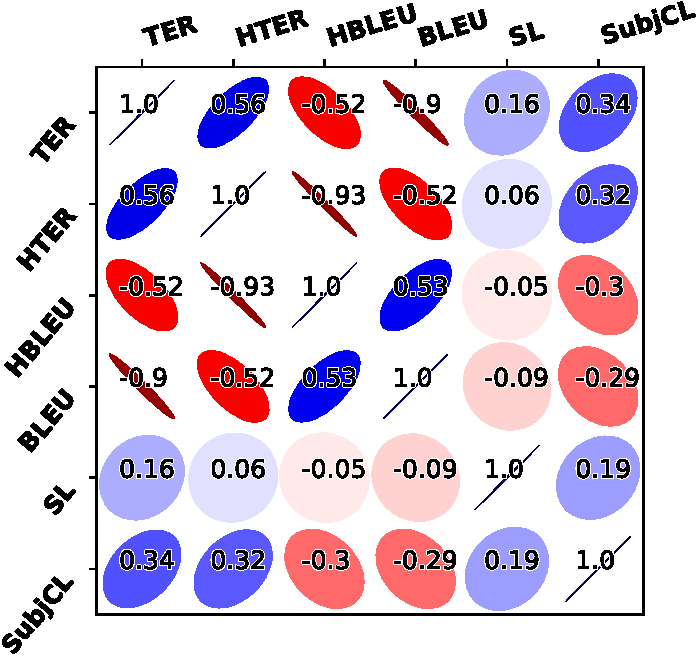
\includegraphics[height=4.5cm]{figures/text-pearson-cropped.pdf}
        \caption{Text -- Pearson}
    \end{subfigure}%
    \begin{subfigure}[b]{0.5\textwidth}\centering
        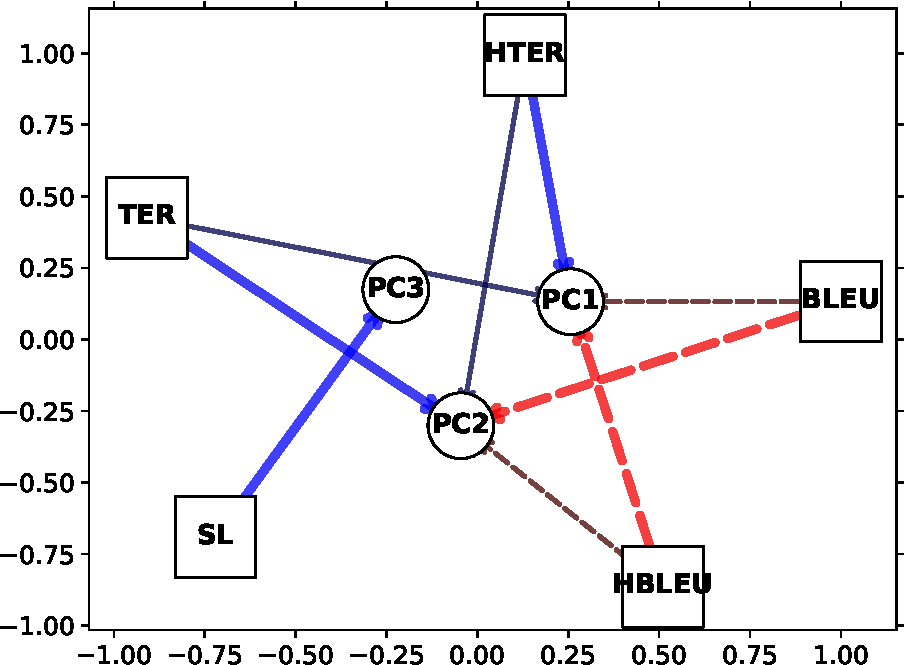
\includegraphics[height=4.5cm]{figures/text-PCA-cropped.pdf}
        \caption{Text -- PCA}
    \end{subfigure}\bigskip\\
    \begin{subfigure}[b]{0.5\textwidth}\centering
        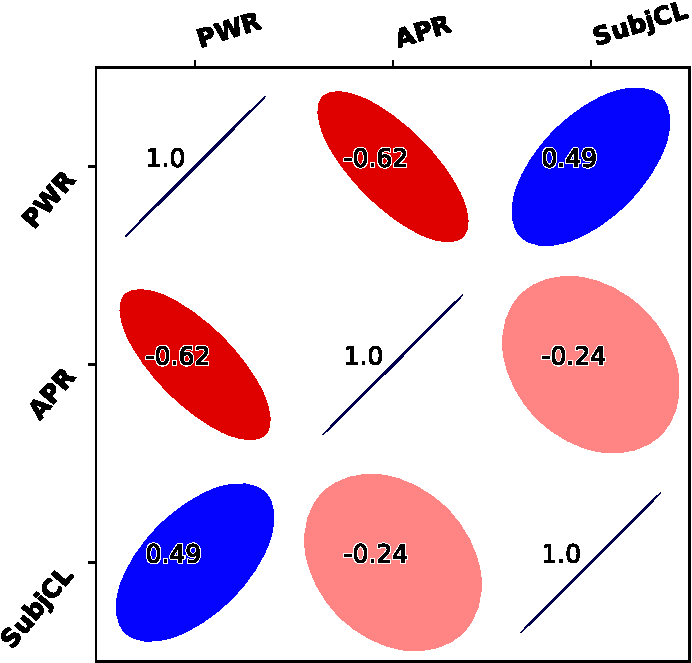
\includegraphics[height=4.5cm]{figures/keyboard-pearson-cropped.pdf}
        \caption{Keyboard -- Pearson}
    \end{subfigure}%
    \begin{subfigure}[b]{0.5\textwidth}\centering
        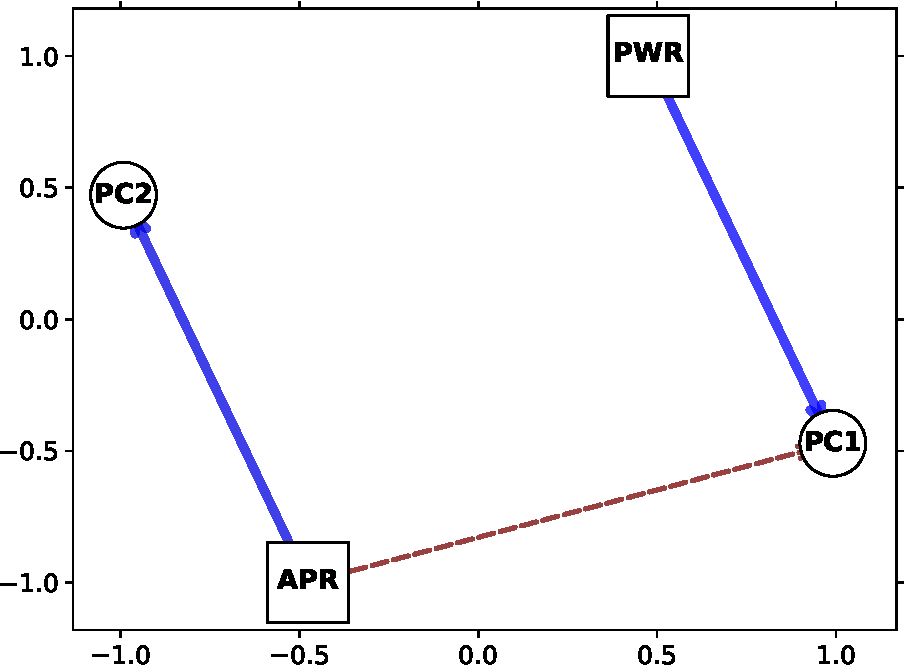
\includegraphics[height=4.5cm]{figures/keyboard-PCA-cropped.pdf}
        \caption{Keyboard -- PCA}
    \end{subfigure}
    \caption{Correlations and PCA for time, text, and keyboard modalities.\label{fig:plotscorrpca1}}
\end{figure}

\begin{figure}
    \begin{subfigure}{0.5\textwidth}\centering
        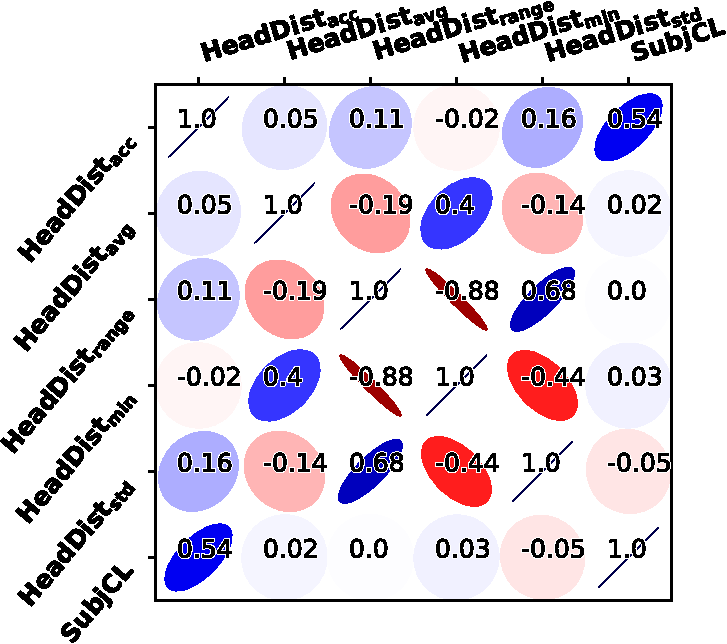
\includegraphics[height=4.5cm]{figures/bodyposture-pearson-cropped.pdf}
        \caption{Body Posture -- Pearson}
    \end{subfigure}%
    \begin{subfigure}{0.5\textwidth}\centering
        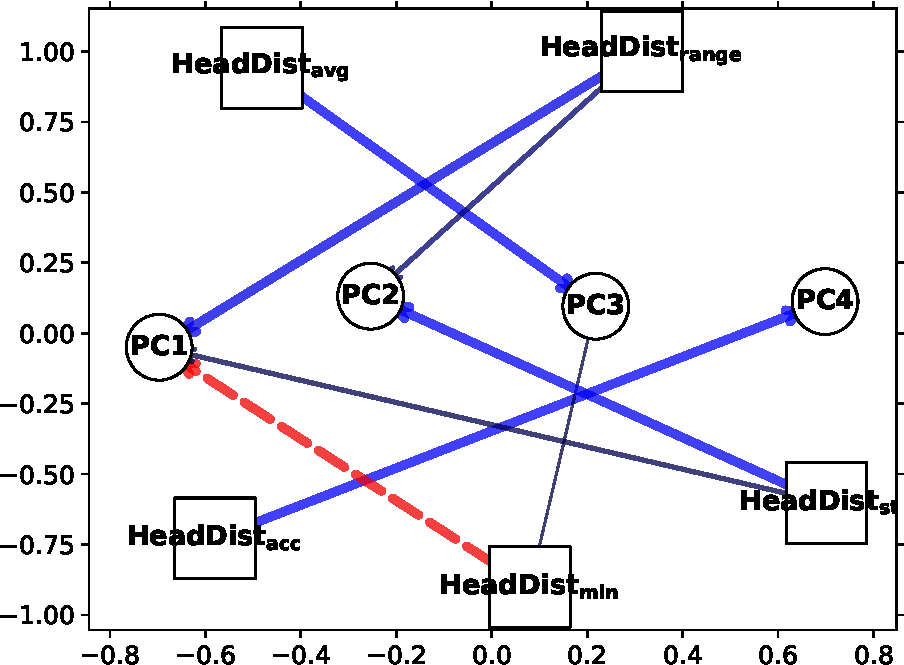
\includegraphics[height=4.5cm]{figures/bodyposture-PCA-cropped.pdf}
        \caption{Body Posture -- PCA}
    \end{subfigure}\bigskip\\
    \begin{subfigure}{0.5\textwidth}\centering
        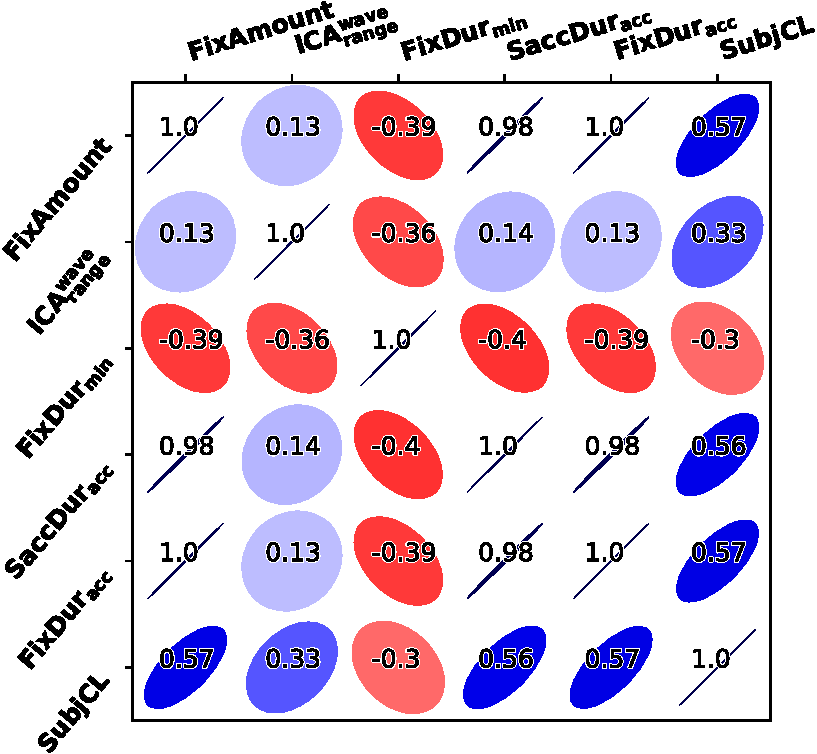
\includegraphics[height=4.5cm]{figures/eyes-pearson-cropped.pdf}
        \caption{Eyes -- Pearson}
    \end{subfigure}%
    \begin{subfigure}{0.5\textwidth}\centering
        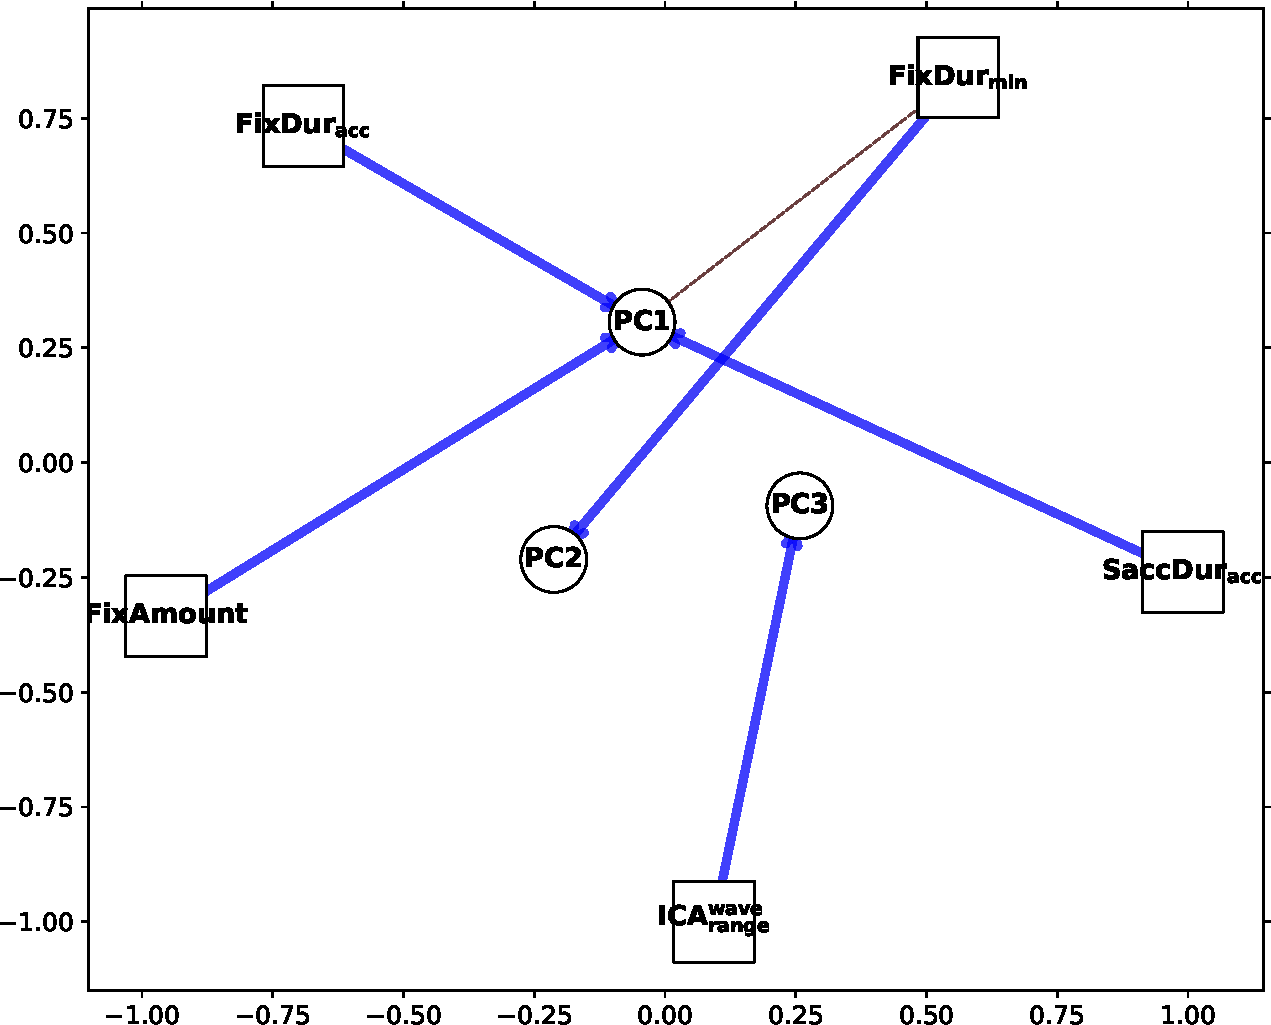
\includegraphics[height=4.5cm]{figures/eyes-PCA-cropped.pdf}
        \caption{Eyes -- PCA}
    \end{subfigure}\bigskip\\
    \begin{subfigure}{0.5\textwidth}\centering
        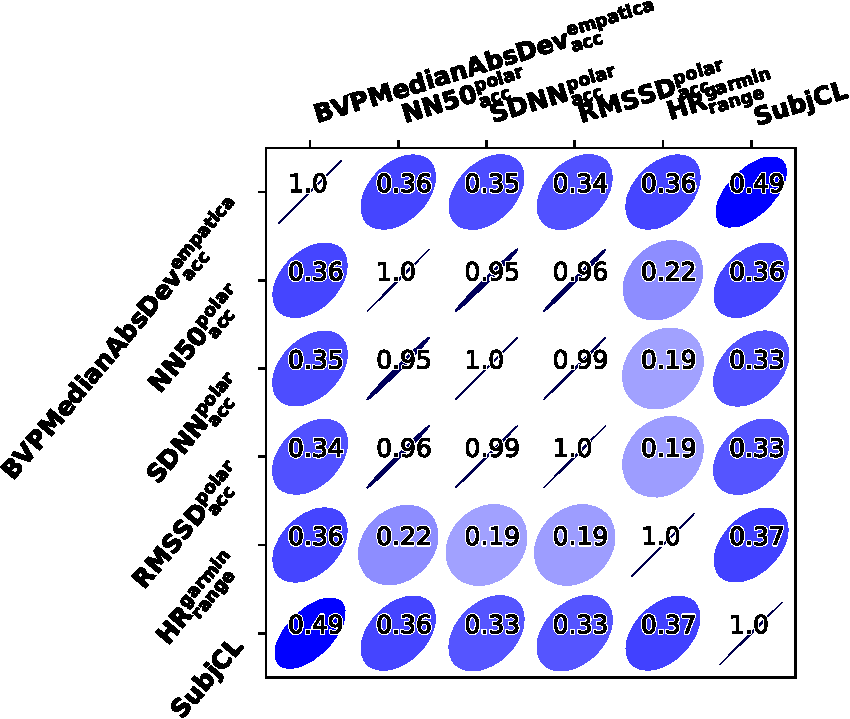
\includegraphics[height=4.5cm]{figures/heart-pearson-cropped.pdf}
        \caption{Heart -- Pearson}
    \end{subfigure}%
    \begin{subfigure}{0.5\textwidth}\centering
        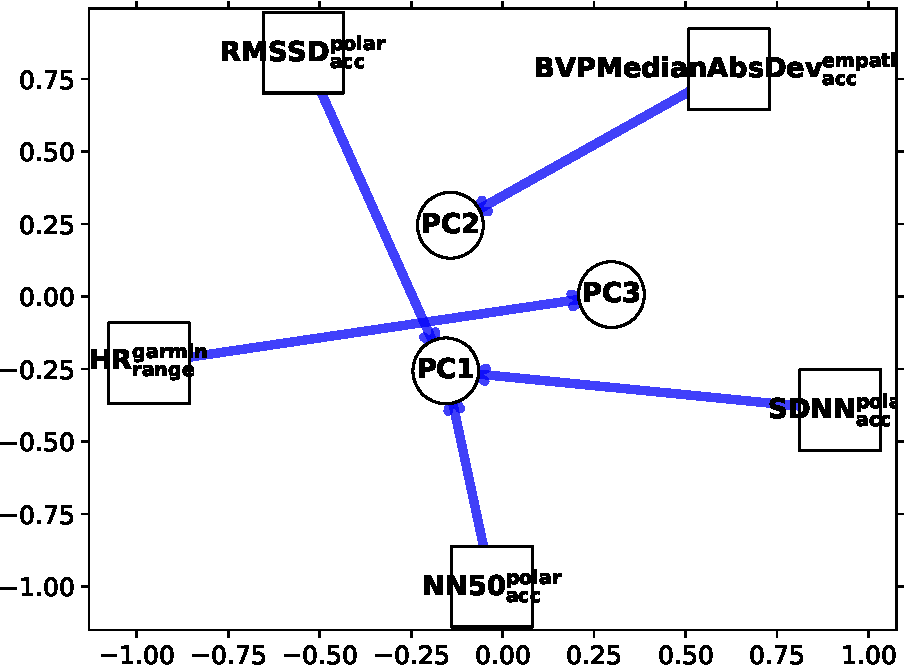
\includegraphics[height=4.5cm]{figures/heart-PCA-cropped.pdf}
        \caption{Heart -- PCA}
    \end{subfigure}
    \caption{Correlations and PCA for body posture, eye, and heart modalities.\label{fig:plotscorrpca2}}
\end{figure}

\begin{figure}
    \begin{subfigure}{0.5\textwidth}\centering
        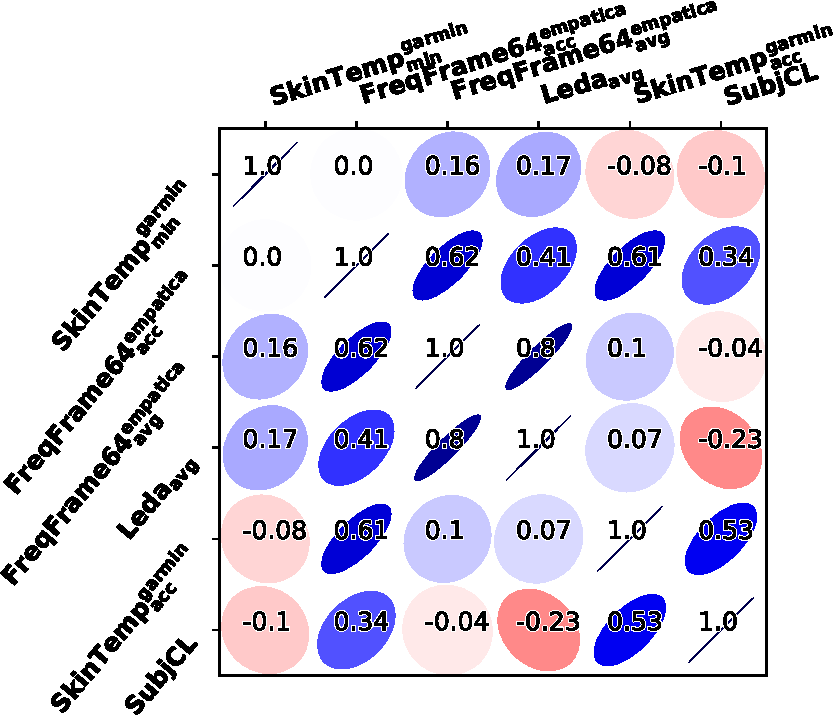
\includegraphics[height=4.5cm]{figures/skin-pearson-cropped.pdf}
        \caption{Skin -- Pearson}
    \end{subfigure}%
    \begin{subfigure}{0.5\textwidth}\centering
        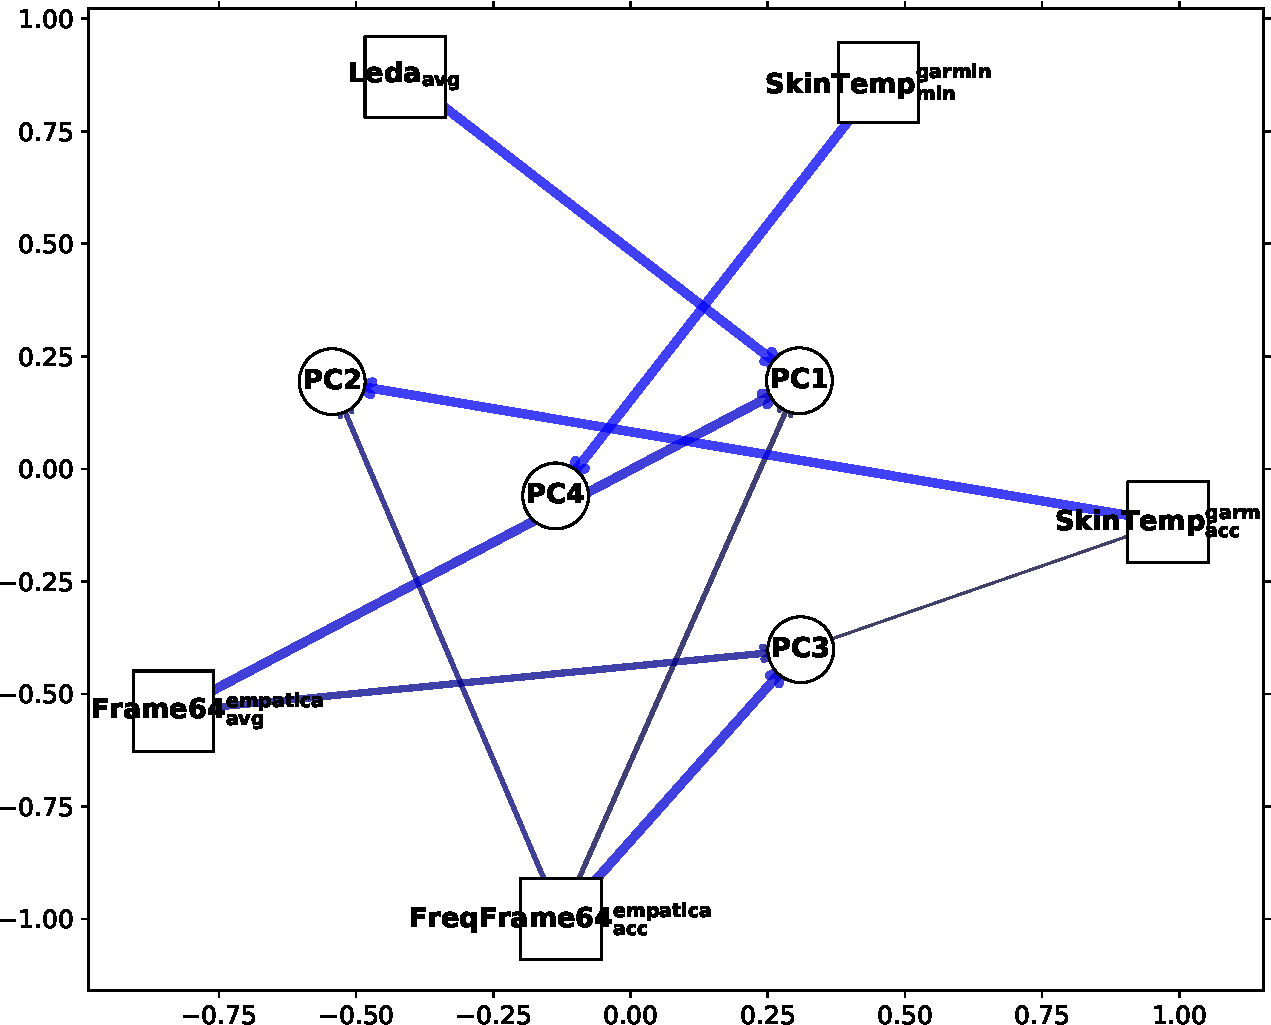
\includegraphics[height=4.5cm]{figures/skin-PCA-cropped.pdf}
        \caption{Skin -- PCA}
    \end{subfigure}\bigskip\\
    \begin{subfigure}{0.5\textwidth}\centering
        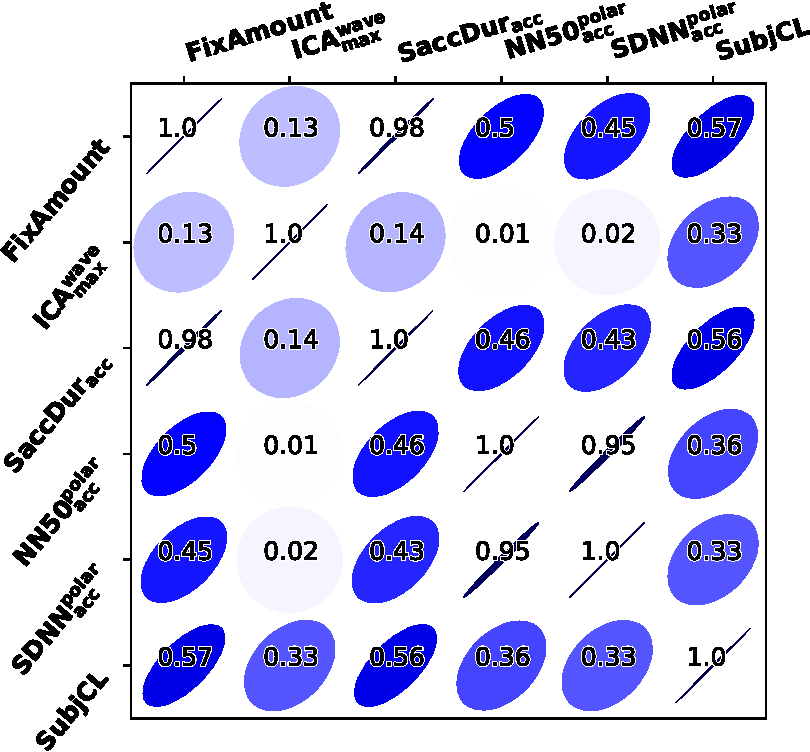
\includegraphics[height=4.5cm]{figures/all-pearson-cropped.pdf}
        \caption{Combined -- Pearson}
    \end{subfigure}%
    \begin{subfigure}{0.5\textwidth}\centering
        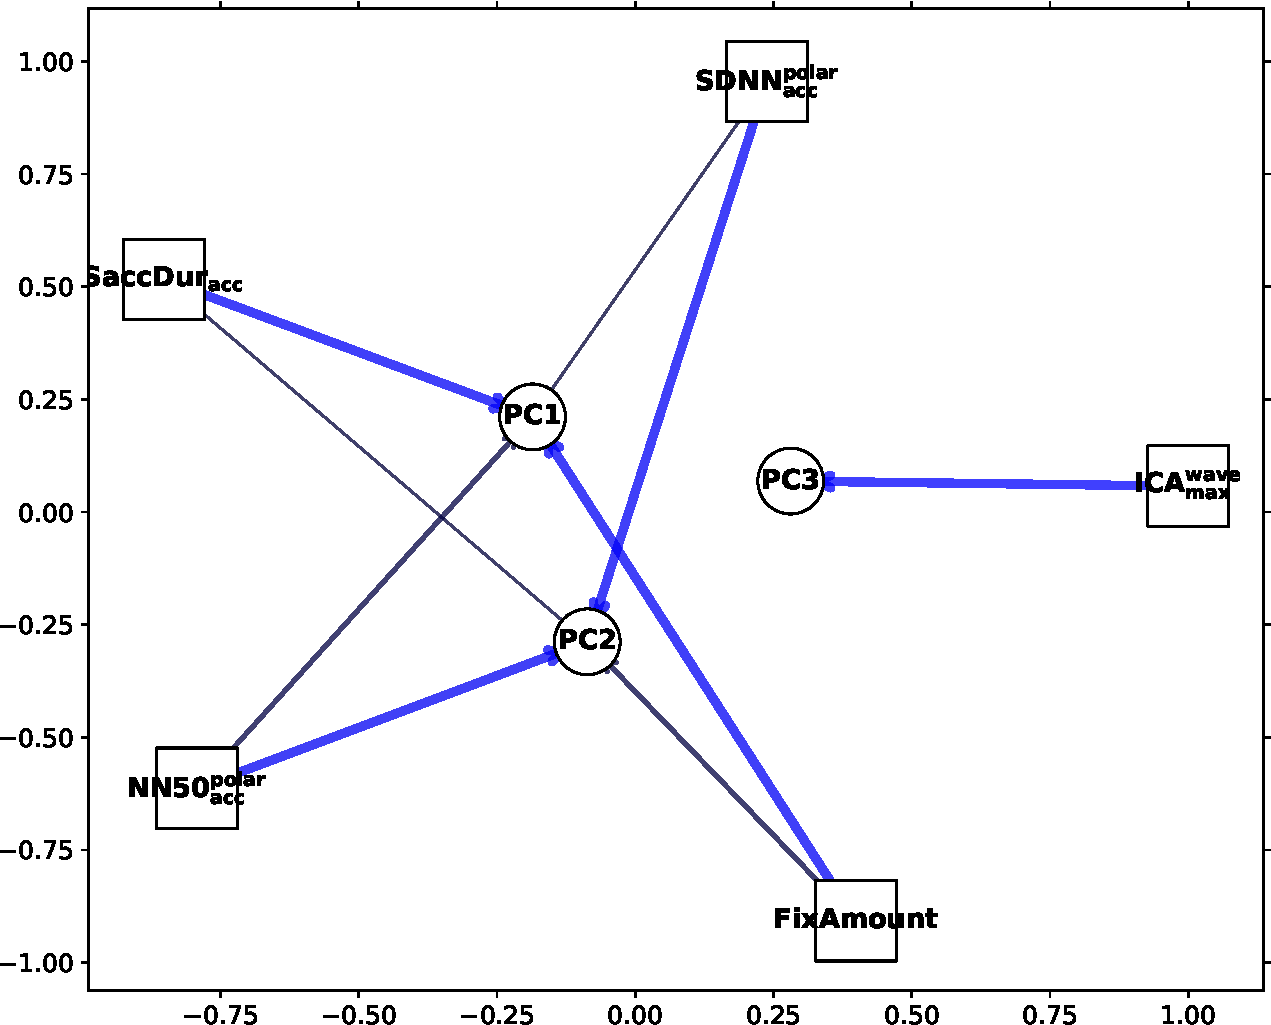
\includegraphics[height=4.5cm]{figures/all-PCA-cropped.pdf}
        \caption{Combined -- PCA}
    \end{subfigure}
    \caption{Correlations and PCA for the skin and combined modalities.\label{fig:plotscorrpca3}}
\end{figure}

Figures~\ref{fig:plotscorrpca1}, \ref{fig:plotscorrpca2} and \ref{fig:plotscorrpca3} depict the pairwise Pearson correlations alongside the PCA loadings, as described above. Narrower ellipses indicate stronger correlations; however, the correlation coefficient is also given numerically and encoded through coloring. Blue and upward-oriented ellipses indicate positive correlations, while red and downward-oriented ellipses indicate negative correlations. The PCA plot shows which feature loads on which PC. Here, the line thickness and color shows the strength of the loading; blue continuous lines represent positive loadings, while red dashed lines indicate negative loadings.
For space reasons, we only summarize the most interesting results, which are all statistically significant.

% Time
For the \textit{time features}, we see that \petime{} and \lnpetime{} correlate very strong\-ly and load on the same PC, but also that both show strong correlations to \subjCL{}. %All correlations are significant after Bonferroni-Holm correction.

% Text
For the \textit{text features}, there expectedly are very strong correlations ($-0.9$) between \ter{} and \bleu{} and between \hter{} and \hbleu{}, where each pair also loads on the same PC. Furthermore, strong correlations can be observed between \ter{} and \hter{}, as well as between \bleu{} and \hbleu{}. %\sentencelength{} shows only very weak relations to all other features and also loads on its own PC.
%All correlations except for \sentencelength{} vs.\ any of \hter{}, \hbleu{}, \bleu{} are statistically significant (p < 0.05) after Bonferroni-Holm correction.

% Keyboard
For the \textit{keyboard features}, we see a very strong correlation between \apr{} and \pwr{}, however, both load on distinct PCs.
\pwr{} correlates more strongly to\linebreak\subjCL{} than \apr{}, indicating that \pwr{} is by itself a better estimator of \subjCL{} than \apr{}.
%and a strong correlation between \pwr{} and \subjCL{}, as well as a moderate correlation between \apr{} and \subjCL{}. This indicates that \pwr{} is by itself a better estimator of \subjCL{} than \apr{}. %All correlations are statistically significant (p < 0.01)% after Bonferroni-Holm correction
%.
%The PCA plot shows that while strong correlations exist, both \apr{} and \pwr{} mostly load on distinct PCs.

% Body Posture
%In contrast to the above features, the \textit{body posture} is a continuous signal, i.e.\ as described above, we calculate 6 simple features on top of the signal, of which the 5 best are reported. All correlations \geq 0.4 are statistically significant (p < 0.05) here. % We find very strong correlations between \headdist{range} and \headdist{min}/\headdist{std} as well as strong correlations between \headdist{acc} and \subjCL{}. Further rather strong correlations can be seen between \headdist{min} and \headdist{std}/\headdist{avg}. While all these correlations are statistically significant (p < 0.05), all other weaker correlations are not significant.
%The PCAs show that the different \headdist{} features load on distinct PCs, with the only strong overlap between \headdist{range} and \headdist{min}.

% Eyes
As expected, the most relevant \textit{eye features} %we can only consider the strongest features selected by feature selection, to keep the results readable.  %I.e.\ \fixamount{}, \ica{wave}{range}, \fixdur{min}, \saccdur{acc}, and \fixdur{acc}, are analyzed.
%As expected,
\fixamount{}, \saccdur{acc}, and\linebreak\fixdur{acc} correlate by almost 1, load on the same PC, and strongly relate to \subjCL{}.%, which makes sense as the amount of fixations obviously impacts the fixation time, which again strongly relates to the saccade duration
%. These three measures also strongly relate to the \subjCL{} and load on the same PC, while the other measures load on different PCs. %We can further see that \ica{wave}{range} also shows moderate correlations to both \subjCL{} and \fixdur{min}.
%All correlations except for \ica{wave}{range} vs.\ \saccdur{acc} and \fixdur{acc} are statistically significant (p < 0.05).

% heart
For the \textit{heart features}, %we again consider only a small subset of important features. T
the correlations between \nn{polar}{acc}, \sdnn{polar}{acc}, and \rmssd{polar}{acc} are again very close to 1, and the PCA plot nicely visualizes that they cluster together. \bvpmedadempatica{} shows the strongest correlation to \subjCL{}. %, and further moderate correlations to the other measures considered.
%\hr{garmin}{range} shows only weak correlations of less than 0.2 to all measures except \subjCL{}. %, which shows shows moderate correlations to all features considered here.
%All correlations in the plot are statistically significant (p < 0.01).

% Skin
Inspecting the most relevant \textit{skin features}, we see very strong correlations between \freqframegsr{64, Empatica}{avg} and \ledalabGlMean{}, as well as medium to strong correlations between the frequency frame and \skintemp{Garmin}{acc} features. %All correlations > 0.17 in the plot are statistically significant (p < 0.05). The PCA plot shows that each feature loads on its separate PC most strongly, but also shows some weaker loadings to the PCs of other features.


% Combined
Most interestingly, for the \textit{combined features} %We see that all features in the plot correlate moderately to strongly to \subjCL{}.
we can again see that \sdnn{polar}{acc} and \nn{polar}{acc}, as well as \fixamount{} and \saccdur{acc}, correlate with almost a value of 1. There also seems to be a strong link between the HRV measures and the eye measures \saccdur{acc} and \fixamount{}. %Here, all correlations > 0.14 are statistically significant (p < 0.01).
The PCA further shows that there is one PC for the HRV measures, one for the \ica{}{}, and another one for the eye features \fixamount{} and \saccdur{acc}.


%\subsection{Detailed Correlation Analysis}
%\todo{write and compare to journal results}


\subsection{Discussion}
Overall, very good regression results of up to 0.7 MSE on a 9-point scale were achieved by our regression models. This amount of error should be acceptable for most possible applications discussed in \cite{herbig2019chi}. %However, further testing on larger datasets including more participants would be necessary to validate this finding.
While the 5 by 2-fold CV results are often slightly worse, which might be because less training data was seen, the results of 1 by 10-fold and 5 by 2-fold are comparable, and the very small standard deviations indicate that the models are rather robust.

% Comparison to MTJ
When comparing the regression results without adding participant and segment to \citet{herbig2019mt}, whose approach is almost the same apart from having fewer sensors and features, we note a few similarities and differences: first of all, we found consistently better results across all modalities; however, already the baseline yields better results on our dataset. %, which indicates that the ratings of our professional participants are a bit more stable around the mean.
While the time features in \citet{herbig2019mt} were rather good, they are among the worst modalities here. A reason might be that we considered many more features, that helped the other modalities improve over the time as a feature.
Furthermore, while in \citet{herbig2019mt} the eyes were by far the best among the three main categories eye, skin, and heart, all three show similar results here. This could be due to the numerous additional skin and heart features considered in our analysis. Whereas in both studies the combined approach leads to the best results, the performance gains when combining multiple modalities were much stronger in \citet{herbig2019mt}, % than they are here,
probably again because the three main categories are already very good by themselves. %That way, the multi-modal approach was not significantly better than the eye, skin, or heart based approaches.

So when we do not consider the individual participant and the segment they are post-editing (Table~\ref{tab:resultsnopartid} or \citealp{herbig2019mt}), we can achieve the best results only with our main categories, eyes, heart, skin, or by combining features from several modalities.
This is relevant for less controlled and more practical applications, e.g.\ adapting the user interface to perceived CL, where it is impossible to use participant and segment information, as ideally no two translators should post-edit the same sentence (which would otherwise be contained in TM).

In contrast, when we do consider participant and segment (Table~\ref{tab:resultspartid}), modalities of lesser quality, like time, text, keyboard, or body posture can also achieve good results. So considering \textit{who is editing what} seems to yield enough information to learn from when combined with these features, while without considering participant and segment, the generalization is impeded. %This is probably due to a strong overfit to the participant and segment, which simplifies the problem considerably.
However, if the goal is to conduct a controlled experiment, e.g.\ to investigate the impact of different sentence features on subjectively felt CL, integrating participant and segment into the models allows to also achieve valuable estimates with these other modalities. The above experiment therefore also suggests that text quality, keyboard, and time measures, which are frequently used in the literature to estimate effort, only work well in controlled settings.

% Comparison to vieira
While we cannot compare all our correlation and PCA results to \citet{vieira2016measures}, since we considered many more features, there is still some interesting overlap:
% Time
The time features in both studies correlated strongly to \subjCL{}.
% Keyboard
Furthermore, the link between the \pwr{} and \subjCL{} also seems comparable, while that between \apr{} and \subjCL{} appears weaker in our dataset. However, the correlation between these two keyboard features is similarly strong in both studies.
% Eyes
The eye features \fixamount{} and \fixdur{} also correlate to a similar extent with \subjCL{} in both studies.
To summarize, we could both reproduce (except \apr{} vs.\ \subjCL{}) and extend the findings by \citet{vieira2016measures}, which strengthens our results.

% Proabably can do better than our feature selection approach by handcrafting based on detailed feature insights.
The correlation and PCA especially revealed that many highly redundant features were selected by the feature selection approach (e.g.\ the HRV measures).
The reason for this probably is their strong correlation to \subjCL{}; however, due to the redundancy, it is unclear whether incorporating multiple such features really helps.
Therefore, we want to explore if handcrafting a set of features with fewer redundancies, or using a more sophisticated feature selection approach than \texttt{RFECV}, could boost the performance further. %As a simple example, the time features which strongly correlate to \subjCL{} and improved the results in \cite{herbig2019mt}, were not selected for the \textit{combined} model.
% Only investigated very few correlations and PCAs
Since space constraints allowed us to analyze only very few features in terms of correlations and PCA, we also plan to investigate the link to the non-selected features, as well as a PCA including more features from all different modalities than the few reported here.
%While space and time constraints allowed us to analyze only a very few features in terms of correlations and PCA, we could still gain many insights and extend the work of \cite{vieira2016measures}. However, much more can and should be analyzed here in the future, in particular the link to the non-selected features, or a PCA including features from all different modalities instead of only the few eye and heart features that were among the best 5 combined features.

% Limitations
\subsection{Limitations}
The results presented in this study are subject to the following limitations: the data sample is relatively small, since only 10 subjects participated in our study.
Next, while we performed CV and only report results on segments unseen during training, we did not completely leave out participants and then predict those participants' perceived CL from the data gathered by the other participants. Thus, to achieve these results in practice one may need to fine-tune and train for new users. %, and one cannot expect the existing model to work immediately.
%Furthermore, the choice of sentences might lead to different results than evaluating the approach in the wild.
Moreover, %our prediction approach is rather indirect: using sensor measurements, we predict the subjectively assessed CL, which we assume to be a good proxy for actual CL based on the literature. While the rating scale used has been utilized in a large variety of experiments, participants may still have had different interpretations of the scale's labels that might have biased the results.
one should also note that our eye tracker only samples at 90\,Hz% (as opposed to 240 Hz)
, which could affect the peak velocity reconstruction and thereby saccades \citep{mack2017effect}.
%Last, while our predictive approach yields interesting first insights and offers a simple and effective way to explore a variety of features, it is only a ``top-down'' approach, which pipes several features into different regression models and applies feature selection to choose an appropriate subset. As discussed above, using the insights from the correlation and PCA analysis to select an optimal set of features, and then tuning the hyper-parameters of a model trained upon these features, might yield better results.
Last, while our predictive approach yields interesting first insights, it is only an automatic ``top-down'' approach that might be improved by selecting an optimal set of features and tuning the hyper-parameters.

% Conclusion and Future Work
\section{Conclusions and future work}
% Summary
In this paper, we have focused on perceived cognitive PE effort and argued for the need to robustly measure CL during PE.
In contrast to most related work, we investigated whether and how multiple modalities to measure CL can be combined and used for the task of predicting the level of perceived CL during PE of MT. %To the best of our knowledge, several of the implemented features have not previously been explored in PE.
%Compared to \cite{herbig2019mt}, we extended their already large set of CL measures even further by incorporating pupil diameter related measures, as well as using the Garmin Forerunner 935 and the Empatica E4 wristband and adding further heart- and skin-related features.
To the best of our knowledge, our analyzed feature set comprises the most diverse set of features from a variety of modalities that has to date been investigated in the translation domain, considering even more factors than \citet{herbig2019mt}.

% Summary of predicitive results
Based on the data gathered from 10 professional translators, we report how well subjective CL can be predicted depending on the various features: %First of all, we find that models trained on any of the investigated modalities are significantly better than a simple baseline.
When the models are unaware of which participant and segment the data belongs to, eye, skin, and heart features, or a combination of different modalities, performed best.
In contrast, for regression models that can react differently depending on participant and segment, the less well performing categories time, text, keyboard, and body posture also achieved good results, probably due to overfitting on the participant. While this finding is very interesting for controlled experiments, it is less relevant for practical use, where no two participants should PE the same segment.
Overall, the trained models can estimate CL during PE without interrupting the actual process through manual ratings with comparably low error of at best 0.7 MSE on a 9-point scale. However, further data analysis is needed to understand the required steps to achieve such results in practice.

% Summary of corr and PCA
We also report how strongly the different measures correlate and which features cluster together, where we reproduce almost all the findings of \citet{vieira2016measures} and extend them further by considering many more features. %However, even more analysis is needed here to really investigate every single of our features% instead of only the ones that performed well on their own
%. %Most interesting about this analysis was, however, that our feature selection approach frequently chose features with strong correlations to \subjCL{}, even if highly correlated features were already contained in the dataset. %, yielding highly redundant choices.

% Improvements
In the future, we want to conduct more detailed investigations, e.g.\ in terms of a more complex feature selection approach or hand-crafting a subset of features based on the correlation and PCA findings, in combination with hyper-parameter tuning, to make better use of the available data than the chosen ``top-down'' regression approach. % chosen for this work.
Furthermore, we want to use the captured continuous signals to already predict perceived CL while still editing the segment (i.e.\ based on a time window of the data), to allow for more real-time applications.
%Currently, all our features are calculated on all data available per segment, which is sufficient to predict perceived CL after finishing the segment. However, as discussed in Section~\ref{sec:datanorm}, all of our continuous features could also be calculated on smaller time intervals, which we want to investigate in the future. %Therefore, in the future we want to investigate whether we can detect the level of CL even before a segment is finished, by calculating running averages instead.

The long-term goal is to be able to decrease the perceived CL, and thereby stress and exhaustion, during PE. As discussed in \citet{herbig2019chi}, this could be achieved by fine-tuning MT systems on the user's CL measurements to produce less demanding outputs, or %by simply intervening in the PE process within CAT tools when high loads are detected, e.g.\
by automatically showing alternative translations or other forms of assistance.
The measurement techniques explored within this paper form the basis for future research towards this goal.



\section*{Acknowledgments}
This research was funded in part by the Deutsche Forschungsgemeinschaft (DFG) under grant number GE 2819/2-1/AOBJ: 636684. The responsibility lies with the authors.

{\sloppy\printbibliography[heading=subbibliography,notkeyword=this]}
\end{document}
